\documentclass[11pt]{report}

\usepackage{style}
\usepackage{math_env}

\usepackage{tikz, pgfplots, pgf-pie}
\usepackage{caption, subcaption}
\usepackage{tikz}
\usepackage{scalerel}
\usepackage{pict2e}
\usepackage{tkz-euclide}
\usepackage{pgfplots, pgfplotstable, pgf-pie}

\usetikzlibrary{calc}
\usetikzlibrary{patterns, arrows}
\usetikzlibrary{shadows}
\usetikzlibrary{external}

\pgfplotsset{compat=newest}
\usepgfplotslibrary{statistics, fillbetween}

\title{Statistica}
\author{Federico Bustaffa}
\date{02/02/2023}

\begin{document}

\maketitle
\tableofcontents

\chapter{Introduzione}

Il corso tratterà le modalità di reperimento e analisi di dati da blockchain tramite Python. Si compirà un'analisi
statistica sui dati raccolti tramite \emph{scraping} o API di vario genere per riuscire ad estrapolare informazioni
sulle blockchain prese in esame.

Saranno necessarie nozioni di statistica descrittiva ed inferenziale e si farà uso di strumenti per l'analisi di
grafi.

Le librerie Python necessarie per lavorare al meglio in questo ambito sono:
\begin{itemize}
	\item \verb|BeautifulSoup|, \verb|Scrapy|: web scraping
	\item \verb|Pandas|: gestione di tabelle
	\item \verb|Numpy|: algebra vettoriale e matriciale
	\item \verb|SciPy|: statistica
	\item \verb|Matplotlib|: visualizzazione di grafici
	\item \verb|NetworkX|: analisi di grafi
\end{itemize}
Per installare le librerie scaricare il package manager \verb|pip| di Python:
\begin{verbatim}
	> sudo apt install python3-pip
\end{verbatim}
Installazione delle librerie
\begin{verbatim}
	> pip install beautifulsoup4
	> pip install scrapy
	> pip install pandas
	> pip install numpy
	> pip install scipy
	> pip install matplotlib
	> pip install networkx
\end{verbatim}

\section{Blockchain}
Una \textbf{blockchain} utilizza un modello computazionale differente dal classico modello \textbf{client-server},
si basa infatti sul sistema \textbf{peer-to-peer}.

In questo modello ogni nodo possiede una frazione del potere necessario a compiere determinate azioni all'interno
della blockchain. Il sistema nasce infatti per eliminare l'entità centrale che controlla e gestisce l'intero servizio.

Possiamo vedere una blockchain come un \textbf{registro} \emph{distribuito} e \emph{replicato} tra i nodi di una
rete \emph{peer-to-peer}. In altre parole ogni nodo della rete possiede una copia della blockchain uguale a quella
di tutti gli altri nodi.

Una proprietà fondamentale al fine di mantenere la blockchain consistente e \textbf{immutabile} è la
\textbf{tamper freeness} garantita tramite meccanismi crittografici e algoritmi basati sul consenso.


\section{Analisi degli errori}
Parliamo ora delle tecniche per l'analisi dell'errore. La continuità della funzione implica che il problema sia
\emph{ben posto}. La relazione
\[
	\ein = \frac{f(\tx) - f(x)}{f(x)} =
	\frac{f(\tx) - f(x)}{\tx - x} \frac{x}{f(x)} \frac{\tx - x}{x}
\]
si ricava che la \emph{differenziabilità} di $f(x)$ è essenziale per il controllo dell'errore inerente. In
particolare se la funzione è \textbf{regolare}, ossia derivabile volte con derivate continue, allora vale
lo sviluppo di Taylor
\[ f(\tx) = f(x) + f'(x) (\tx - x) + \frac{f''(\xi)}{2} (\tx - x)^2 \]
con $|\xi - x| \leq |\tx - x|$, da cui si ottiene
\[
	\ein \frac{f(\tx) - f(x)}{f(x)} \doteq \frac{f'(x)}{f(x)} \cdot x \cdot \epsilon_x = c_x \cdot \epsilon_x
\]
\begin{definition}
	La quantità
	\[ c_x = c_x (f) = \frac{f'(x)}{f(x)} \cdot x \]
	è detta \textbf{coefficiente di amplificazione} e fornisce una misura del condizionamento del problema.
\end{definition}

Più in generale possiamo dire che se $f : \Omega \to \R$ è definita su un insieme aperto di $\R^n$, differenziabile
due volte su $\Omega$ ed il segmento di estremi $\tx$ e $x$ è contenuto in $\Omega$ allora vale
\[
	\ein = \frac{f(\tx) - f(x)}{f(x)} \doteq
	\frac{1}{f(x)} \sum_{i=1}^n \frac{\partial f}{\partial x_i} (x) x_i \epsilon_{x_i} =
	\sum_{i=1}^n c_{x_i} (f) \epsilon_{x_i}
\]
con
\[ c_{x_i} (f) = \frac{1}{f(x)} \frac{\partial f}{\partial x_i} (x) x_i \]
con $1 \leq i \leq n$, detti coefficienti di amplificazione della funzione $f$ rispetto alla variabile $x_i$.

\part{Probabilità}

\chapter{Probabilità e indipendenza}
Il calcolo delle \textbf{probabilità} ci serve per la costruzione di un modello
\textbf{statico inferenziale}, il quale unisce statistica descrittiva e probabilità per descrivere
la realtà.

Prima di addentrarci nei formalismi matematici introduciamo qualche concetto \emph{primitivo}.
\begin{itemize}
	\item Quello che vogliamo calcolare è la probabilità che un certo \textbf{evento} accada. Il
	      concetto
	      di evento non si può formalizzare, ma possiamo fare qualche esempio: se lanciamo un dado,
	      il fatto che esca 6 è un evento.
	\item Il secondo concetto è quello di \textbf{casuale} o \textbf{aleatorio}
	      (\textbf{stocastico}). Queste tre parole hanno quasi lo stesso significato ma possiamo
	      generalizzare dicendo che significano \emph{"dovuto al caso"}. Più avanti introdurremo
	      altri termini come \emph{variabili aleatorie} e \emph{indipendenza stocastica}.
\end{itemize}
Due dei problemi che andremo a trattare sono:
\begin{itemize}
	\item La \textbf{rappresentazione} degli eventi.
	\item Quali \textbf{proprietà} devono soddisfare le probabilità.
\end{itemize}
Per riuscire a capire meglio tutti questi concetti sarà necessario anche conoscere qualche nozione
di base sulle serie.

\section{Spazi di probabilità}
Possiamo vedere tutti gli eventi possibili come un insieme, detto \textbf{spazio campionario}, che
indicheremo con $\Omega$.
\begin{itemize}
	\item $\Omega$ rappresenta lo \textbf{spazio campionario} di tutti i possibili eventi.
	\item I sottoinsiemi di $\Omega$ sono detti \textbf{eventi}.
	\item I singoli esiti appartenenti ad un insieme sono detti \textbf{eventi elementari}
\end{itemize}
Dato che possiamo vedere gli spazi campionari come insiemi di eventi, è facile trovare una
correlazione tra le operazioni insiemistiche e i connettivi logici.
\begin{itemize}
	\item All'unione ($A \cup B$) corrisponde un \verb|or| logico.
	\item All'intersezione ($A \cap B$) corrisponde un \verb|and| logico.
	\item Alla complementazione ($A^c$) corrisponde un \verb|not| logico.
	\item Alla differenza ($A \backslash B$) corrisponde $A \land \lnot B$
	\item La relazione insiemistica di sottoinsieme ($A \subseteq B$) corrisponde
	      all'implicazione logica. Se accade $A$ allora accade $B$.
	\item Se $A \cap B = \emptyset$ allora si dice che gli eventi sono \textbf{disgiunti}.
\end{itemize}
Ora possiamo gestire gli eventi legati da connettivi logici tramite operazioni insiemistiche
equivalenti.

\begin{example}
	Se lanciamo un dado a 6 facce abbiamo
	\[ \Omega = \{ 1, 2, 3, 4, 5, 6 \} \]
	L'insieme degli eventi tali che il numero uscito sia
	\begin{itemize}
		\item Pari è $A = \{ 2, 4, 6 \}$
		\item Maggiore di 3 è $B = \{ 4, 5, 6 \}$
		\item Non pari è $A^c = \{ 1, 3, 5 \}$
		\item Pari o maggiore di 3 è $A \cup B = \{ 2, 4, 5, 6 \}$
		\item Pari e maggiore di 3 è $A \cap B = \{ 4, 6 \}$
		\item Pari ma non maggiore di 3 è $A \backslash B = A \cap B^c = \{2\}$
		\item Sia pari che dispari è $A \cap A^c = \emptyset$
	\end{itemize}
\end{example}

\subsection{Funzione di probabilità}
Vogliamo ora definire la probabilità su una classe \emph{ammissibile} di eventi. Questo non è
sempre possibile. Si vuole quindi definire una classe ammissibile che sia chiusa per le operazioni
insiemistiche viste in precedenza.

\begin{definition}
	Sia $\Omega \neq \emptyset$ e $\F \subseteq \mathcal{P}(\Omega)$ una famiglia di sottoinsiemi
	di $\Omega$. Diciamo che $\F$ è un'\textbf{algebra di parti} se
	\begin{itemize}
		\item $\Omega, \emptyset \in \F$
		\item $\F$ è stabile per la complementazione: se $A \in \F$ allora $A^c \in \F$
		\item $\F$ è stabile per unione finita, ovvero se $A_1, A_2, ..., A_n \in \F$ allora
		      anche la loro unione $\cup_{i=1}^n A_i$ appartiene a $\F$.
	\end{itemize}
	Se inoltre $\Omega$ e una sua algebra di parti $\F$ hanno infiniti elementi, diciamo che $\F$
	è una $\sigma$\textbf{-algebra} se soddisfa l'ipotesi addizionale:
	\begin{itemize}
		\item $\F$ è stabile per unione numerabile, ovvero se esiste una successione di
		      sottoinsiemi $A_1, A_2, ...$ appartiene a $\F$ anche la loro unione
		      $\cup_{i=1}^\infty A_i$ appartiene a $\F$.
	\end{itemize}
\end{definition}

La $\sigma$-algebra è quindi un'operazione chiusa per tutte le operazioni insiemistiche viste
sopra ed è la classe degli eventi \emph{ammissibili}.

La \textbf{probabilità} di un evento $A \in \F$ è il grado di fiducia che $A$ si realizzi ed è
compreso tra 0 e 1.

\`E intuitivo supporre che, se due eventi $A$ e $B$ sono disgiunti, allora la probabilità che si
realizzi $A \cup B$ è $P(A) + P(B)$. Questo equivale a dire che la probabilità è una funzione
d'insieme \textbf{finitamente additiva}.

\begin{definition}
	Dato $\Omega$ un insieme e $\F$ una $\sigma$-algebra di $\Omega$, la \textbf{probabilità} è
	una funzione
	\[ P : \F \to [0, 1] \]
	tale che
	\begin{itemize}
		\item L'evento certo ha probabilità unitaria: $P(\Omega) = 1$.
		\item Se la successione degli $A_i$ è una successione di elementi di $\F$ a due a due
		      disgiunti, si ha, nel caso in cui la successione sia finita, che
		      \[ P \left( \bigcup_{i=1}^n A_i \right) = \sum_{i=1}^n P(A_i) \]
		      Se invece la successione è infinita allora vale
		      \[
			      P \left( \bigcup_{i=1}^{+\infty} A_i \right) = \sum_{i=1}^{+\infty} P(A_i) =
			      \lim_{n \to +\infty} \sum_{i=1}^n P(A_i)
		      \]
		      Questa proprietà è detta $\sigma$\textbf{-additività}.
	\end{itemize}
\end{definition}

\begin{definition}
	La terna $(\Omega, \F, P)$ formata da uno spazio campionario, una $\sigma$-algebra ed una
	probabilità $P$ definita su $\F$ viene chiamata \textbf{spazio di probabilità}.
\end{definition}

\paragraph{Proprietà} La probabilità, così come l'abbiamo definita, comporta che
\begin{itemize}
	\item $P(\emptyset) = 0$
	\item $P(A^c) = 1 - P(A)$
	\item $P(A \backslash B) = P(A) - P(B)$
	\item $P(A \cup B) = P(A) + P(B) - P(A \cap B)$
	\item $P(A \cup B \cup C) = P(A) + P(B) + P(C) -
		      P(A \cap B) - P(A \cap C) - P(B \cap C) + P(A \cap B \cap C)$
\end{itemize}

\begin{proposition}
	Supponiamo di avere una successione infinita $A \in \F$	allora
	\begin{itemize}
		\item $A$ è una successione \textbf{crescente}, cioè $A_i \subseteq A_{i+1}$, $\forall i$
		      se vale
		      \[ A = \cup_{i=1}^\infty A_i \]
		\item $A$ è una successione \textbf{decrescente}, cioè $A_{i+1} \subseteq A_i$,
		      $\forall i$ se vale
		      \[ A = \cap_{i=1}^\infty A_i \]
	\end{itemize}
	In entrambi i casi vale
	\[ P(A) = \lim_{i \to \infty} P(A_i) \]
\end{proposition}

\begin{definition}
	Se $P(A) = 0$ si dice che $A$ è un evento \textbf{trascurabile}.
\end{definition}

\begin{definition}
	Se $P(A) = 1$ si dice che $A$ è un evento \textbf{quasi certo}.
\end{definition}

Facciamo ora qualche considerazione sulla $\sigma$-algebra. Consideriamo $\Omega$ finito o
numerabile e quindi così formato
\[ \Omega = \{ \omega_1, \omega_2, ..., \omega_i, ... \} \]
allora possiamo prendere $\F = \mathcal{P}(\Omega)$ e la probabilità è univocamente determinata
da $p_i = P(\{ \omega_i \})$. Vale infatti che
\[ P(A) = \sum_{\omega_i \in A} p_i \]
Quindi, nel caso $A$ abbia un numero
\begin{itemize}
	\item finito di elementi, $P(A)$ equivale alla somma dei $p_i$.
	\item infinito di elementi, $P(A)$ equivale alla serie dei $p_i$.
\end{itemize}

\begin{example}
	Vogliamo definire un modello di probabilità per la scelta casuale di un punto sull'intervallo
	$[a,b]$ in modo che la scelta sia uniforme. In questo caso abbiamo che $\Omega$ è non
	numerabile in quanto esistono infiniti punti tra $a$ e $b$. Ne segue che la probabilità di
	scegliere un punto in questo intervallo con una funzione di probabilità definita come in
	precedenza non può che essere 0.

	Potrebbe venirci in mente di definire la probabilità di scegliere un punto $x$ all'interno di
	$[a,b]$ come la lunghezza dell'intervallo ($b-a$) ma ci si può facilmente accorgere che non
	si riesce a definire in modo coerente la lunghezza di ogni sottoinsieme di $[a,b]$.

	Per questo si introduce una $\sigma$-algebra più \emph{piccola} di $\mathcal{P}(\Omega)$,
	detta degli \textbf{insiemi misurabili}.
\end{example}

\subsubsection{Serie}
Andiamo ora a capire trattare alcuni concetti di base, relativi alle serie, necessarie ad
inquadrare meglio la situazione.

\begin{definition}
	Sia $a_1, a_2, \dots$ una successione di termini, e sia
	\[ s_n = a_1 + \dots + a_n \]
	la somma parziale dei primi $n$ termini. Definiamo quest'ultima come \textbf{serie} se esiste
	il limite delle somme parziali
	\[ \sum_{n=1}^\infty a_n = \lim_{n \to \infty} \sum_{k=1}^n a_k = \lim_{n \to \infty} s_n \]
	Se esiste finito questo limite si dice che la serie \textbf{converge}.
\end{definition}

\begin{observation}
	Da qui è facile osservare che
	\[ a_n = s_n - s_{n-1} \]
	ed è chiaro che se esiste il limite
	\[ \lim_{n \to \infty} s_n \]
	il valore $a_n$ tende a zero per $n \to \infty$ ma non è vero il viceversa.
\end{observation}

Supponiamo ora il caso in cui $a_n \geq 0$ per ogni $n \in \N$ allora le somme parziali crescono
\[ s_n \leq s_{n+1} \]
In questo caso ha sempre senso parlare di limite poiché, per una successione del genere, vale
\[ \sum_{n=1}^\infty = \lim_{n \to \infty} \sum_{k=1}^n a_k \in [0, +\infty]  \]
Il fatto che esista sempre il limite non significa che la serie converga. Come detto poco fa, la
serie converge se il limite tende ad un numero reale finito.

\begin{definition}
	Consideriamo la serie
	\[ \sum_{n=1}^\infty |a_n| \]
	Se il limite per $n \to \infty$ tende ad un numero reale finito si dice che la serie converge
	\emph{assolutamente}.
\end{definition}

\begin{theorem}
	Se una serie converge assolutamente allora converge.
\end{theorem}

Per le serie di termini positivi che convergono assolutamente vale anche una sorta di proprietà
\textbf{associativa} in cui si partizionano gli indici della serie in sottoinsiemi di $\N$
($A_1, A_2, \dots$) e vale
\[ \sum_{n=1}^\infty a_n = \sum_{n=1}^\infty \left( \sum_{k \in A_n} a_k \right) \]

Consideriamo ora due serie fondamentali di cui non facciamo la dimostrazione ma che ci saranno
molto utili in futuro:
\begin{itemize}
	\item \textbf{Serie geometrica}: se $|a| < 1$ allora vale
	      \[ \sum_{n=0}^\infty a^n = 1 + a + a^2 + \dots = \frac{1}{1 - a} \]
	\item \textbf{Sviluppo in serie dell'esponenziale}
	      \[ e^x = \sum_{n=0}^\infty \frac{x^n}{n!} \]
\end{itemize}

\section{Spazio degli eventi}
Possiamo vedere tutti gli eventi possibili come un insieme, detto \textbf{spazio degli eventi} o
\textbf{universo}, che indicheremo con $\Omega$.
\begin{itemize}
	\item $\emptyset$, $\Omega$ sono spazi di eventi.
	\item Se $A$ e $B$ sono spazi di eventi, lo sono anche $A \cup B$ (rappresenta un \verb|or| logico di
	      eventi), $A \cap B$ (rappresenta un \verb|and| logico di eventi) e $A^c$ (rappresenta un
	      \verb|not| logico di eventi). Questi possono essere sottoinsiemi di $\Omega$ o $\Omega$ stesso.
\end{itemize}

\begin{example}
	Lanciamo un dado
	\[ \Omega = \{ 1, 2, 3, 4, 5, 6 \} \]
	L'insieme degli eventi tali che il numero uscito sia
	\begin{itemize}
		\item Pari $A = \{ 2, 4, 6 \}$
		\item Maggiore di 3 $B = \{ 4, 5, 6 \}$
		\item Non pari $A^c = \{ 1, 3, 5 \}$
		\item Pari o maggiore di 3 $A \cup B = \{ 2, 4, 5, 6 \}$
		\item Pari e maggiore di 3 $A \cap B = \{ 4, 6 \}$
	\end{itemize}
\end{example}

\begin{definition}
	Quando c'è un insieme di eventi $\A$ con queste proprietà:
	\begin{itemize}
		\item $\emptyset, \Omega \in \A$
		\item Se $A \in \A$ allora $A^c \in \A$
		\item Se $A, B \in \A$ allora $(A \cup B) \in \A$ e $(A \cap B) \in \A$
	\end{itemize}
	questo è chiamato \textbf{algebra di parti}.
\end{definition}

\begin{definition}[Provvisoria]
	Definiamo la \textbf{probabilità} come una funzione
	\[ P : \A \to [0, 1] \]
	tale che
	\begin{itemize}
		\item $P (\Omega) = 1$.
		\item $A \cap B = \emptyset$ allora $P(A \cup B) = P(A) + P(B)$.
	\end{itemize}
	Una funzione con queste proprietà è detta \emph{finitamente additiva}.
\end{definition}

Vediamo alcune conseguenze di questa definizione
\begin{itemize}
	\item $P(\emptyset) = 0$
	\item $P(A^c) = 1 - P(A)$
	\item Se $B \subseteq A$ e consideriamo $A \backslash B = A \cap B^c$ allora
	      \[ P(A \backslash B) = P(A) - P(B) \]
	\item $P(A \cup B) = P(A) + P(B) - P(A \cap B)$
\end{itemize}
Ancora qualche definizione
\begin{itemize}
	\item Se $P(A) = 0$ si dice che $A$ è un evento \textbf{trascurabile}.
	\item Se $P(A) = 1$ si dice che $A$ è un evento \textbf{quasi certo}.
\end{itemize}
Introduciamo anche un altro concetto, ossia quello di \textbf{additività numerabile} o
$\sigma$-\textbf{additività}, necessaria per \emph{andare al limite} (sarà chiaro più avanti), senza la
quale non si potrebbe fare calcolo statistico. Se consideriamo una successione di eventi a due a due
disgiunti del tipo
\[ A_1, \; A_2, \; A_3, \; \dots \]
con $A_i \cap A_j = \emptyset$ se $i \neq j$ allora deve valere
\[
	P(\cup_{n=1}^\infty A_n) = \sum_{n=1}^\infty P(A_n) =
	\lim_{n \to \infty} \sum_{k=1}^n P(A_k) = 	\lim_{n \to \infty} P(A_1) + \dots + P(A_n)
\]
Questa è detta \textbf{somma infinita}.

\begin{definition}
	Definiamo la \textbf{probabilità} come la funzione $P$ definita sugli eventi
	\[ P : eventi \to [0, 1] \]
	dove $P(\Omega) = 1$ e
	\[ P(\cup_{n=1}^\infty A_n) = \sum_{n=1}^\infty P(A_n) \]
\end{definition}

Siamo ora in grado di capire meglio cosa significa \emph{andare al limite}. Sia
$A_1 \subseteq A_2 \subseteq A_3 \dots$ una successione di eventi, abbiamo che l'evento $A$ definito come
l'unione infinita della successione, equivale a
\[ A = \cup_{n=1}^\infty A_n = \lim_{n \to \infty} A_n \]
Vale quindi che la probabilità che $A$ si verfichi equivale a
\[ P(A) = \lim_{n \to \infty} P(A_n) \]
Il punto di partenza è il caso in cui $\Omega$ è finito ed è quindi definito come segue
\[ \Omega = \{ \omega_1, \dots, \omega_n \} \]
e dunque possiamo prendere come probabilità la funzione finitamente additiva definita su tutto lo spazio
degli eventi tale che $P(\Omega) = 1$. In particolare, quando $\Omega$ è finito allora la probabilità si
può sempre definire su tutti i suoi sottoinsiemi, come la somma della probabilità dei punti che lo
costituiscono
\[ P(A) = \sum_{\omega_i \in A} P(\omega_i) = \sum_{\omega_i \in A} p_i \]
Se invece $\Omega$ è infinito ma numerabile, per esempio $\Omega = \N$. Quando $\Omega$ è numerabile allora
la probabilità si può definire su tutti i sottoinsiemi di $\Omega$ e basta conoscere la probabilità dei
singoli punti $p_i$
\[ p_i = P(\omega_i) \]
e deve valere
\[ \sum_{i=1}^\infty p_i = 1 \]
mentre se consideriamo un sottoinsieme $A$ di $\Omega$ allora vale
\[ P(A) = \sum_{\omega_i \in A} p_i \]

\chapter{Calcolo combinatorio}
Il calcolo combinatorio è un elemento fondamentale alla base del calcolo delle probabilità. Non ci
soffermiamo più di tanto su questo aspetto ma cerchiamo di fare nostro qualche concetto utile.

\section{Distribuzione uniforme}
Se $\Omega$ è finito e tutti i suoi punti sembrano ragionevolmente equiprobabili, allora vale
\[ P(\omega_i) = \frac{1}{n} \]
Questa è chiamata \textbf{distribuzione uniforme} di probabilità e vale
\[ P(A) = \frac{\# A}{\# \Omega} = \frac{\text{casi favorevoli}}{\text{casi possibili}} \]
Se $\Omega$ è infinito non possiamo parlare di distribuzione uniforme.

\subsection{Nozioni di calcolo combinatorio}
A questo punto è necessario introdurre alcuni concetti fondamentali necessari a comprendere meglio
ciò che andremo a fare più avanti. Il calcolo combinatorio si occupa di proporre dei metodi per
raggruppare gruppi di elementi e, per ogni metodo, vuole contare il numero di possibili
raggruppamenti.

I metodi che andiamo a trattare possono tenere conto dell'ordine con il quale gli elementi sono
raggruppati oppure no. Ogni metodo ha una sua versione in cui si tiene conto delle possibili 
ripetizioni degli elementi.

\subsubsection{Combinazioni}
Le \textbf{combinazioni} contano il numero di sottoinsiemi di $k$ elementi estratti da un insieme di
$n$ elementi senza tener conto dell'ordine.

\begin{definition}
	Definiamo la \textbf{combinazione senza ripetizione} come il numero di sottoinsiemi di $k$ elementi,
	ognuno estratto una sola volta, da un insieme di $n$ elementi.
	\[ \binom{n}{k} = \frac{n!}{k! (n-k)!} = \frac{n (n-1) \dots (n-k+1)}{k!} \]
	La notazione $\binom{n}{k}$ indica il \textbf{coefficiente binomiale}.
\end{definition}

\begin{definition}
	Definiamo la \textbf{combinazione con ripetizione} come il numero di sottoinsiemi di $k$ elementi,
	dove ogni elemento può essere estratto $k$ volte da un insieme di $n$ elementi.
	\[ \binom{n+k-1}{k} = \frac{(n + k - 1)!}{k! (n-1)!} \]
\end{definition}

\subsubsection{Disposizioni}
Le \textbf{disposizioni} contano il numero di possibili sequenze ordinate di $k$ elementi estratte da 
un insieme di $n$ elementi.

\begin{definition}
	Definiamo la \textbf{disposizione senza ripetizione} come il numero di sequenze ordinate di $k$
	elementi, estratta da un insieme di $n$ elementi. In questo caso i $k$ elementi sono tutti diversi
	ma vengono contati tutti i possibili modi di riordinare la stessa sequenza.
	\[ \frac{n!}{(n - k)!} \]
\end{definition}

\begin{definition}
	Definiamo la \textbf{disposizione con ripetizione} come il numero di sequenze ordinate di $k$
	elementi, estratta da un insieme di $n$ elementi. In questo caso i $k$ elementi possono ripetersi
	fino a $k$ volte
	\[ n^k \]
\end{definition}

\subsubsection{Permutazioni}
Le \textbf{permutazioni} contano in quanti possibili modi si può riordinare un insieme di $n$ elementi.

\begin{definition}
	Definiamo la \textbf{permutazione senza ripetizione} come il numero di modi in cui si possono ordinare
	$n$ elementi tutti diversi.
	\[ n! \]
\end{definition}

\begin{definition}
	Definiamo la \textbf{permutazione con ripetizione} come il numero di modi in cui è possibile riordinare
	$n$ elementi nel caso in cui $k$ di essi siano ripetuti.
	\[ \frac{n!}{n_1! \cdot n_2! \cdot ... \cdot n_k!} \]
	In questa formula $n_i$ è il numero di volte che l'elemento $i$ è ripetuto all'interno della sequenza.
\end{definition}

\subsubsection{Binomio di Newton}
Uno strumento interessante di cui non facciamo la dimostrazione ma che ci sarà utile più avanti è il
\textbf{binomio di Newton}.

\begin{definition}
	Definiamo il \textbf{binomio di Newton} come
	\[ (a + b)^n = \sum_{k=0}^n \binom{n}{k} \cdot a^k b^{n-k} \]
\end{definition}


\section{Probabilità condizionata}
La \textbf{probabilità condizionata} indica la probabilità che si verfichi un evento sapendo che
se ne verifica un altro.

\begin{example}
	Supponiamo di lanciare un dado equilibrato e supponiamo di sapere che l'esito è un numero
	pari. Sapendo ciò, vogliamo sapere quale sia la probabilità che l'esito sia maggiore o uguale
	di 4. Consideriamo i due insiemi $A$ e $B$ così definiti.
	\[ A = \{ 4, 5, 6 \} \quad B = \{ 2, 4, 6 \} \]
	Vogliamo sapere qual'è la probabilità di estrarre dall'insieme $B$ un numero maggiore o uguale
	di 4. \`E immediato che la risposta debba essere $2/3$ dato che
	\[
		\frac{2}{3} = \frac{\# (A \cap B)}{\# B} =
		\frac{\# (A \cap B) / \# \Omega}{\# B / \# \Omega} =
		\frac{P(A \cap B)}{P(B)}
	\]
\end{example}

\begin{definition}
	Dato uno spazio di probabilità $(\Omega, \F, P)$ e un evento non trascurabile $B$, definiamo
	\textbf{probabilità condizionata} di $A$ dato $B$, come
	\[ P(A | B) = \frac{P(A \cap B)}{P(B)} \]
	Essa indica la probabilità che accada $A$ sapendo che accade $B$.
\end{definition}

Dalla formula segue che se $A$ e $B$ sono eventi e $B$ è non trascurabile, allora
\[ P(A \cap B) = P(A | B) \cdot P(B) \]
e vale una formula più generale data dalla seguente proposizione.

\begin{proposition}
	Siano $A_1, A_2, \dots, A_n$ eventi la cui intersezione è non trascurabile, allora
	\[
		P(A_1 \cap  \dots \cap A_n) = P(A_1) P(A_2 | A_1) P(A_3 | A_1 \cap A_2)
		\dots P(A_n | A_1 \cap \dots \cap A_{n-1})
	\]
\end{proposition}

\begin{definition}
	Siano $B_1, \dots, B_n$ eventi non trascurabili che formano una partizione dello spazio
	campionario $\Omega$, se
	\[ B_i \cap B_j = \emptyset \quad \land \quad B_1 \cup \dots \cup B_n = \Omega \]
	per ogni $i,j$ con $i \neq j$, allora sono detti \textbf{sistema di alternative}.
\end{definition}

\begin{theorem}[Fattorizzazione]\label{th: fattorizzazione}
	Sia $B_1, \dots, B_n$ un sistema di alternative, allora vale
	\[ P(A) = \sum_{i=1}^n P(A | B_i) \cdot P(B_i) \]
	Per ogni evento $A \in \F$.
	\begin{proof}
		Se partizioniamo $\Omega$ in $n$ alternative e poi definiamo un insieme
		$A \subseteq \Omega$, possiamo vedere $A$ in questo modo
		\[ A = \cup_{i=1}^n (A \cap B_i) \]
		ossia come l'unione disgiunta dei pezzi di $A$ che stanno nei vari $B_i$. Quindi vale che
		\[ P(A) = \sum_{i=1}^n P(A \cap B_i) = \sum_{i=1}^n P(A | B_i) P(B_i) \]
	\end{proof}
\end{theorem}

Generalmente questa formula si applica in casi in cui $P$ non è nota a priori ma sono note le
probabilità condizionate relative ad un sistema di alternative.

\begin{example}
	Ci sono 2 urne, la prima con 5 biglie rosse e 5 blu, la seconda con 8 biglie rosse e 2 blu.
	Scegliamo casualmente una delle due urne e da questa estraiamo una biglia e ne osserviamo il
	colore. Vogliamo calcolare la probabilità che esca una biglia rossa. In questo esempio lo
	spazio campionario è il seguente
	\[ \Omega = \{ (\text{urna}, \text{colore biglia}) \} \]
	dove
	\[ \text{urna} \in \{ 1, 2 \} \quad \text{colore biglia} \in \{ r, b \} \]
	A questo punto noi sappiamo che la probabilità di scegliere una delle due urne è
	\[ P(1) = P(2) = \frac{1}{2} \]
	La seconda informazione di cui siamo a conoscienza è che se scegliamo l'urna 1 abbiamo 5
	biglie rosse e 5 blu e quindi
	\[ P(r | 1) = \frac{5}{10} = \frac{1}{2} \]
	Se invece scegliamo l'urna 2 abbiamo 8 biglie rosse e quindi
	\[ P(r | 2) = \frac{8}{10} = \frac{4}{5} \]
	A questo punto siamo in grado di calcolare la probabilità complessiva di estrarre una biglia
	rossa ricavandola con il teorema di fattorizzazione \ref{th: fattorizzazione} in questo modo
	\[ P(r) = P(r | 1) \cdot P(1) + P(r | 2) \cdot P(2) = \frac{13}{20} \]
\end{example}

\begin{example}
	Un test diagnostico per una data malattia ha un indice di sensibilità di $0.99$ per una
	persona malata, ossia, da esito positivo con probabilità $0.99$. E ha indice di specificità
	$0.97$, ossia, da esito negativo con probabilità $0.97$ per una persona sana.

	Supponendo che l'1\% della popolazione soffra di tale malattia, vogliamo calcolare la
	probabilità che il test, su un individuo a caso, dia esito positivo. Si applica la formula di
	fattorizzazione al sistema di alternative $B_1 = \{ \text{sano} \}$ e
	$B_2 = \{ \text{malato} \}$ e all'evento $A = \{ \text{test positivo} \}$. Svolgendo i calcoli
	in modo analogo a prima otteniamo che
	\[ P(A) = 0.0396 \]
\end{example}

\begin{theorem}[Bayes]\label{th: bayes}
	Siano $A$ e $B$ eventi non trascurabili. Allora vale
	\[ P(B | A) = \frac{P(A | B) \cdot P(B)}{P(A)} \]
	In particolare se $B_1, B_2, \dots, B_n$ allora vale
	\[
		P(B_i | A) = \frac{P(A | B_i) \cdot
			P(B_i)}{\displaystyle\sum_{j=1}^n P(A | B_j) \cdot P(B_j)}
	\]
	per ogni $i = 1, \dots, n$.
	\begin{proof}
		La dimostrazione è molto semplice basta infatti notare che
		\[
			P(B | A) = \frac{P(B \cap A)}{P(A)} =
			\frac{P(A \cap B)}{P(A)} = \frac{P(A | B) \cdot P(B)}{P(A)}
		\]
		La seconda formula segue dalla prima dove $B=B_i$ e dalla formula di fattorizzazione
		per $P(A)$.
	\end{proof}
\end{theorem}

La formula di Bayes viene usata per \emph{invertire} il condizionamento tipicamente in contesti
in cui accade un evento $A$ riferito a un'\emph{osservabile} e vogliamo dedurre la probabilità di
un'alternativa $B_i$ di eventi \emph{causa}.

\begin{example}
	Facendo riferimento all'esempio di prima delle biglie, supponiamo di estrarre una biglia
	rossa e vogliamo calcolare la probabilità che questa sia stata estratta dalla prima urna.
	\[
		P(1 | r) = \frac{P(r | 1) P(1)}{P(r)} =
		\frac{\frac{5}{10} \cdot \frac{1}{2}}{\frac{13}{20}} = 0.385
	\]
\end{example}

\begin{example}
	Facendo riferimento al test diagnostico, supponiamo che il test dia esito positivo e vogliamo
	calcolare la probabilità che la persona sia effettivamente malata.
	\[
		P(\text{malato} | \text{positivo}) =
		\frac{P(\text{positivo} | \text{malato}) \cdot
			P(\text{malato})}{P(\text{positivo})} = 0.25
	\]
\end{example}

Come possiamo notare, si fa riferimento a casi in cui la probabilità condizionata nel membro di
destra dell'equazione è già nota.
\section{Indipendenza}
Il concetto di \textbf{indipendenza} nasce dalla necessità di esprimere in modo rigoroso che la
probabilità di un evento $A$ non cambia sapendo che accade $B$ e viceversa. Per $A$ e $B$ non
trascurabili vale quindi 
\[ P(A) = P(A | B) \quad \Leftrightarrow \quad P(A) P(B) = P(A \cap B) \]
Lo stesso vale per $P(B)$.

\begin{definition}
	Due eventi $A$ e $B$ sono \textbf{indipendenti} se
	\[ P(A \cap B) = P(A) P(B) \]
\end{definition}

Si può dimostrare per esercizio che, se $A$ e $B$ sono indipendenti allora lo sono anche
\begin{itemize}
	\item $A^c$ e $B$
	\item $A$ e $B^c$
	\item $A^c$ e $B^c$
\end{itemize}
L'indipendenza è dunque stabile per la complementazione. Si può inoltre dimostrare che 
\begin{itemize}
	\item Se $P(A) \in \{ 0, 1 \}$ allora $A$ è indipendente da ogni altro evento.
	\item Se $A \cap B = \emptyset$ allora $A$ e $B$ non sono indipendente a meno che $P(A)$ o
		$P(B)$ siano 0.
\end{itemize}

\begin{example}
	Si vuole estrarre una carta da un mazzo di 40 carte napoletane
	\[ \Omega = \{ \text{carte} \} \]
	Ci chiediamo se i due eventi 
	\[ A = \{ \text{asso} \} \quad B = \{ \text{denari} \} \]
	sono indipendenti. La probabilità di estrarre un asso equivale a
	\[ P(A) = \frac{4}{40} = \frac{1}{10} \]
	La probabilità di estrarre una carta di denari è invece
	\[ P(B) = \frac{10}{40} = \frac{1}{4} \]
	La probabilità di estrarre l'asso di denari equivale a 
	\[ P(A \cap B) = \frac{1}{40} = \frac{1}{10} \cdot \frac{1}{4} = P(A) P(B) \]
	Quindi gli eventi sono indipendenti.
\end{example}

\section{Probabilità sulla retta reale}
In questo paragrafo vedremo due classi principali di esempi di probabilità su $\Omega = \R$.
Queste due classi non esauriscono i possibili esempi di probabilità su $\R$ ma saranno l'oggetto
delle applicazioni che vedremo.

\subsection{Probabilità discreta}
Una \textbf{probabilità discreta} su $\Omega = \R$ è una probabilità su $\Omega = \R$, prendendo
come $\sigma$-algebra le parti di $\R$ ($\F (\mathcal{P}(\R))$), che sia concentrata su una
successione finita o numerabile $x_1, x_2, \dots$ di punti.

Ad esempio la probabilità associata al numero di volte che esce testa in due lanci di moneta è
una probabilità discreta, concentrata su $\{0,1,2\}$. Chiamiamo $p_i = p(x_i) = P(x_i)$, allora
vale che
\begin{equation}\label{eq: 3.1} P(A) = \sum_{x_i \in A} p(x_i) \end{equation}

\begin{definition}
	La funzione
	\[ p : \{ x_1, x_2, \dots \} \to [0,1] \]
	con $p(x_i) = P(\{x_i\})$ si dice \textbf{funzione di massa} o \textbf{densità discreta} di $P$.
\end{definition}

\begin{observation}
	Facciamo ora alcune osservazioni:
	\begin{itemize}
		\item $p$ soddisfa
		      \[ p(x_i) \geq 0 \quad \land \quad \sum_i p(x_i) = P(\R) = 1\]
		\item Viceversa, data una successione $x_1, x_2, \dots$ finita o numerabile e una funzione
		      $p$ con le proprietà descritte sopra, allora esiste un'unica probabilità $P$ su $\R$
		      avente $p$ come funzione di massa.
		\item Dalla formula \ref{eq: 3.1}, è possibile calcolare $P(A)$ partendo dalla successione
		      degli $x_i$ e dalla funzione di massa.
		\item Si definisce $p$ su tutto $\R$, ponendo $p(x) = 0$ per $x \neq x_i$.
	\end{itemize}
\end{observation}

\subsection{Probabilità con densità}
Prima di parlare di questa classe di probabilità dobbiamo enunciare il seguente teorema:
\begin{theorem}
	Esiste una $\sigma$-algebra $\F \subseteq P(\R) \neq P(\R)$ tale che
	\[ (a, b) \in \F \]
	tali che $-\infty \leq a < b \leq +\infty$ ed esiste $\lambda : \F \to [0, +\infty]$ che sia
	$\sigma$-additiva e tale che, per ogni $-\infty \leq a < b \leq +\infty$,
	\[ \lambda((a,b)) = \lambda((a,b]) = \lambda ([a,b)) = \lambda([a,b]) = b - a \]
\end{theorem}

Chiameremo gli elementi di $\F$ \textbf{insiemi misurabili}. Intersecando tutti gli elementi di
$\F$ con l'intervallo $[0,1]$ otteniamo i sottoinsiemi misurabili di quest'ultimo, che sono una
$\sigma$-algebra sulla quale possiamo definire la probabilità
\[ P (A) = \lambda (A) \]
per ogni $A \subset [0,1]$ misurabile, in modo che
\[ P((a, b)) = |b-a|, \quad \forall a,b \in [0,1] \]

\begin{observation}
	Osserviamo che $\lambda$ assegna lunghezza nulla ai singoli punti, ovvero
	\[ \lambda(x) = \lambda([x,x]) = x - x = 0 \]
	e lo stesso vale per ogni sottoinsieme $A \subset \R$ con al più numerabili elementi.
\end{observation}

\begin{definition}
	Si chiama \textbf{densità di probabilità} sulla retta reale, una funzione non negativa
	$f : \R \to [0, +\infty)$, integrabile e tale che
	\[ \int_{-\infty}^{+\infty} f(x) dx = 1 \]
	Ad ogni densità di probabilità si associa un'unica probabilità sulla $\sigma$-algebra degli
	insiemi misurabili di $\R$ definita da:
	\[ \forall A \in \F, \quad P(A) = \int_A f(x) dx \]
\end{definition}

Perché questa sia una buona definizione si deve controllare che $P$, così definita, soddisfi
\[ P(\R) = \int_\R f(x) dx = 1 \]
per ipotesi, ed inoltre se $A \cap B = \emptyset$ si ha che
\[ P(A \cup B) = \int_{A \cup B} f(x) dx = \int_A f(x) dx + \int_B f(x) dx = P(A) + P(B) \]
Se $X$ ha densità $f$, allora vale
\[ P(X = t) = P_X (t) = \int_{\{t\}} f(x) dx = 0 \]
per ogni $t \in \R$.

\chapter{Variabili aleatorie}
Introduciamo ora le variabili aleatorie. Esse sono, di fatto sono
\textbf{caratteristiche quantitative} dell'esperimento in esame. In questa prima parte seguiranno
qualche definizione ed esempi utili alla comprensione.

\begin{example}
	Si effettuano $n$ lanci di una moneta equilibrata ed essere interessati solo alle volte che
	esce testa. Per riuscire a farlo potremmo assegnare a testa il valore 1 e a croce il valore 0.
	Di conseguenza otteniamo che il numero di volte che esce croce è
	\[ X(a_1, a_2, \dots, a_n) = \sum_{i=1}^n a_i \]
	dove gli $a_i$ sono gli esisti di ogni lancio.
\end{example}

\section{Legge di una variabile aleatoria}
Iniziamo ora a dare qualche definizione per formalizzare meglio il concetto di variabile aleatoria
e perché sono state introdotte.

\begin{definition}
	Dato uno spazio di probabilità $(\Omega, \F, P)$, si dice \textbf{variabile aleatoria} una
	funzione
	\[ X : \Omega \to \R \]
	tale che, per ogni $A \subseteq \R$ misurabile, allora vale
	\[ X^{-1}(A) \in \F \]
\end{definition}

\begin{example}
	Si effettuano $n$ lanci di una moneta equilibrata e otteniamo:
	\[ A = (a_1, \dots, a_n) \]
	Vogliamo ora considerare
	\begin{itemize}
		\item numero di teste: $X(A) = \sum_{i=1}^n a_i$
		\item numero di croci: $Y(A) = n - X(A)$
		\item coppie consecutive testa: $Z(A) = \sum_{i=1}^{n-1} a_i \cdot a_{i+1}$
	\end{itemize}
\end{example}

\begin{definition}
	Per ogni $A \subseteq \R$ misurabile, definiamo
	\[ \{ X \in A \} = X^{-1}(A) = \{\omega \in \Omega | X(\omega) \in A \} \]
	la controimmagine di $A$ tramite $X$.
\end{definition}

Più informalmente, $P_X$ esprime la distribuzione del carattere $X$ nell'esperimento.

\begin{example}
	Si effettuano $n$ lanci di moneta e consideriamo $X$ come il numero di volte che esce testa.
	\[ X(A) = a_1 + \dots + a_n \]
	L'insieme $\{ X \in \{ 0, 1 \} \}$ è l'insieme di casi in cui, per $n$ lanci di moneta,
	otteniamo al massimo una testa. La probabilità di avere al massimo una testa
	la esprimiamo come
	\[ P_X (\{0,1\}) = P (\{X \in \{0,1\}\}) \]
\end{example}

\begin{proposition}
	Dalle considerazioni fatte segue che $P_X : \F \to \R$ è una probabilità su $(\R, \F)$, dove
	$\F$ è l'insieme dei misurabili, verifica quindi
	\begin{itemize}
		\item $P_X (\R) = 1$
		\item $P_X(\cup_{i=1} A_i) = \sum_{i=1} P_X(A_i)$ con $A_1, A_2, ... \subseteq \R$
		      misurabili a due a due disgiunti.
	\end{itemize}
\end{proposition}

\begin{definition}
	Definiamo \textbf{legge di probabilità} o \textbf{distribuzione} di $X$, come
	\[ P_X (A) = P(\{ X \in A\}) \]
	con $A \subseteq \R$ misurabile.
\end{definition}

\begin{example}
	Si effettuano 2 lanci di una moneta equilibrata
	\[ \Omega = \{ 0, 1 \}^2 \]
	e consideriamo $X$ come il numero di volte che esce testa. Quanto vale $P_X$?
	Come possiamo notare, $P_X$ è concentrata su $\{ 0, 1, 2 \}$.
	\[
		P_X (0) = \frac{1}{4} \quad \quad
		P_X (1) = \frac{1}{2} \quad \quad
		P_X (2) = \frac{1}{4}
	\]
	Possiamo quindi dire che $P_X$ è la distribuzione del carattere $X$ all'interno
	dell'esperimento.
\end{example}

\begin{definition}
	Diciamo che $X$ e $Y$ sono \textbf{equidistribuite} se hanno la stessa legge, ovvero se
	\[ P_X = P_Y \]
\end{definition}

Le variabili aleatorie altro non sono che una notazione, che diventa conveniente nel momento in cui
vogliamo considerare più caratteri di un esperimento (e quindi più variabili aleatorie).

E nel momento in cui è necessario svolgere operazioni matematiche tra variabili aleatorie (ad
esempio sommandole).

\begin{observation}
	Data $\tilde{P}$, probabilità su $(\R, \F)$, allora esiste uno spazio $\Omega$ e una variabile
	aleatoria $X : \Omega \to \R$ avente $\tilde{P}$ come legge ($P_X = \tilde{P})$.
\end{observation}

\begin{observation}
	Se c'è un'unica variabile aleatoria $X$, è equivalente considerare $X$ oppure $P_X$.
\end{observation}

\subsection{Tipi di variabili aleatorie}
Possiamo distinguere due classi di variabili aleatorie a seconda della loro legge.

\begin{definition}
	Una variabile aleatoria $X$ è detta \textbf{discreta} se $X(\Omega)$ è finita o numerabile, o
	in modo equivalente, se la sua legge $P_X$ è discreta.
\end{definition}

Per quanto visto sulle probabilità discrete, $P_X$ è determinata dalla sua funzione di massa,
ovvero
\[ P_X (x_i) = P(X = x_i) \]
vale infatti che
\[ P(\{X \in A\}) = P_X (A) = \sum_{x_i \in A} P_X (x_i) \]

\begin{definition}
	Una variabile aleatoria $X$ è detta \textbf{con densità} o \textbf{assolutamente continua} se
	$P_X$ ammette densità di probabilità $f$, ossia
	\[ P(\{X \in A\}) = P_X (A) = \int_A f(x) dx \]
\end{definition}

\begin{example}
	Consideriamo il caso dell'estrazione di un individuo $\omega$ da una popolazione. Supponiamo
	quindi che $\Omega$ rappresenti la popolazione italiana e che
	\begin{itemize}
		\item $X(\omega)$ equivale al numero di figli di $\omega$ (carattere discreto).
		\item $Y(\omega)$ equivale all'altezza di $\omega$ (carattere continuo).
	\end{itemize}
	Abbiamo che
	\[ P_X(x_i) = P(X = x_i) = \frac{\# \{ w | X(w) = x_i\} }{\# \Omega} \]
	ossia la frequenza relativa di $X = x_i$ su tutta la popolazione. $P_X(2)$ è quindi la
	frequenza relativa, sulla popolazione italiana, delle persone con 2 figli.

	Per quanto riguarda $Y$, l'area sottesa da $f$ nell'intervallo $[a,b]$ equivale a
	\[
		\int_a^b f(x) dx = P (a \leq X \leq b)
		= \frac{\# \{ \omega | X(\omega) \in [a,b] \}}{\# \Omega}
	\]
	ossia la frequenza relativa di $X \in [a,b]$ su tutta la popolazione.
\end{example}
\section{Funzione di ripartizione e quantili}
\section{Variabili aleatorie notevoli}
In questa sezione trattiamo le distribuzione di probabilità su $\R$ indispensabili per trattare
ogni applicazione. Si tratta sempre di variabili discrete o definite tramite densità.

\subsection{Variabili binomiali}
Consideriamo come primo caso le \textbf{variabili binomiali} prendendo $n$ prove ripetute, con
esito (per ciascuna prova) successo o insuccesso (schema di Bernoulli) e sia $p$ la probabilità di
successo (nella singola prova).
\[ P(a_1, \dots, a_n) = p^{\# \{i | a_i=1\}} \cdot (1-p)^{\# \{ i | a_i=0 \}} \]
Sia $X$ la variabile aleatoria che conta il numero di successi, ossia
\[ X(a_1, \dots, a_n) = \sum_{i=1}^n a_i \]
Come possiamo notare $X$ è discreta a valori in $\{0,1,2,\dots,n\}$ e ha funzione di massa
\[ P_X(h) = P(X = h) = \binom{n}{h} \cdot p^h \cdot (1-p)^{n-h} \]
con $h \in \{ 0, 1, \dots, n \}$. Possiamo tradurre tutto questo nella probabilità che abbiamo di
avere $h$ successi.

Una \textbf{variabile aleatoria binomiale} di parametri $n \in \N^+$ e $p \in (0,1)$, è tale se
possiede la funzione di massa appena descritta ed è indicata con $B(n, p)$.

\begin{observation}
	Per $n=1$ si parla di variabile aleatoria di Bernoulli e si indica con $B(p)$.
\end{observation}

\begin{example}
	Su 5 lanci di un dado equilibrato, qual è la probabilità che il 6 appaia almeno 2 volte? Per
	prima cosa definiamo $X$ come il numero di volte che esce 6 nelle 5 prove. Vogliamo quindi
	calcolare la probabilità che il 6 esca almeno 2 volte in 5 lanci. Per farlo ci conviene passare
	al problema complementare:
	\[ P(X \geq 2) = 1 - (P(X = 0) + P(X = 1)) \]
	Calcoliamo quindi $P(X=0)$ e $P(X=1)$:
	\begin{gather*}
		P(X = 0) = \binom{5}{0} \cdot \left(\frac{1}{6}\right)^0 \cdot
		\left(1 - \frac{1}{6}\right)^5 = \left(\frac{5}{6}\right)^5 \\
		P(X = 1) = \binom{5}{1} \cdot \left(\frac{1}{6}\right)^1 \cdot
		\left(1 - \frac{1}{6}\right)^4 = \left(\frac{5}{6}\right)^4
	\end{gather*}
	Siamo ora in grado di calcolare $P(X \geq 2)$ come
	\[ P(X \geq 2) = 1 - \left( \left(\frac{5}{6}\right)^5 + \left(\frac{5}{6}\right)^4 \right) \]
\end{example}

\subsection{Variabili geometriche}
Rimaniamo nel contesto delle prove ripetute indipendenti con esito successo o insuccesso. Sia $X$
la variabile aleatoria che rappresenta l'istante del primo successo (l'istante è il numero della
prova). Come possiamo notare, $X$ è discreta a valori in $\N^+ = \{ 1, 2, \dots \}$ e la sua
funzione di massa vale
\[ P(X = h) = (1-p)^{h-1} \cdot p \]
Questo ci dice la probabilità che abbiamo di ottenere il primo successo dopo $h$ tentativi.

Una \textbf{variabile aleatoria geometrica} di parametro $p \in (0,1)$, è tale se possiede la
funzione di massa appena descritta ed è indicata con $G(p)$.

\begin{proposition}[Assenza di memoria]
	Data una variabile geometrica di parametro $p$, per ogni $n,h \in \N^+$, vale
	\[ P(X = n + h | X > n) = P(X = h) \]
	La probabilità di successo dopo $h$ prove non cambia sapendo che il successo non si è
	verificato nelle prime $n$ prove.
\end{proposition}

\subsection{Variabili di Poisson}
Una variabile aleatoria $X$ si dice \textbf{variabile aleatoria di Poisson} di parametro
$\lambda > 0$ se è una variabile aleatoria discreta a valori in $\N$, con funzione di massa
\[ P(X = h) = \frac{\lambda^h}{h!} \cdot e^{-\lambda} \]
con $h \in \N$ e si indica con $P(\lambda)$. La variabile di Poisson conta il numero di
\emph{eventi rari}, infatti, tale variabile aleatoria, approssima una binomiale di parametri $n$ e
$p$ quando $n$ è grande, $p$ è piccola e $\lambda \approx np$. Si può dimostrare infatti che, detta
\[ p^{(n)} (h) = \binom{n}{h} \cdot p_n^h \cdot \left( 1-p_n \right)^{n-h} \]
la funzione di massa di $B(n, p_n)$, con $p_n = \lambda / n$, allora
\[ \lim_{n \to +\infty} p^{(n)} (h) = P_\lambda (h) = \frac{\lambda^h}{h!} \cdot e^{-\lambda} \]
per ogni $h \in \N$.

\begin{example}
	Il numero di clienti ad un dato sportello è descritto da una variabile di Poisson di parametro
	$\lambda = 2.3$. Qual è la probabilita di avere al massimo 2 clienti?
	\begin{align*}
		P(X \leq 2) = & P(X = 0) + P(X = 1) + P(X = 2)                          \\
		=             & \frac{2.3^0}{0!} e^{-2.3} + \frac{2.3^1}{1!} e^{-2.3} +
		\frac{2.3^2}{2!} e^{-2.3}
	\end{align*}
\end{example}

\subsection{Variabili uniformi su un intervallo}
Una variabile aleatoria $X$ è detta \textbf{uniforme} su un intervallo $(a, b)$ dato, se ha densità
\[
	f(x) = \begin{cases}
		\dfrac{1}{b - a} & x \in (a, b)    \\[2ex]
		0                & x \notin (a, b)
	\end{cases}
\]
Una variabile aleatoria uniforme su $(a,b)$ rappresenta la posizione di un punto scelto a caso
senza preferenze sull'intervallo $(a, b)$.

\subsection{Variabili aleatorie esponenziali}
Una variabile aleatoria $X$ è detta \textbf{esponenziale} di parametro $\lambda > 0$ se ha densità
\[
	f(x) = \begin{cases}
		\lambda \cdot e^{-\lambda x} & x > 0    \\[2ex]
		0                            & x \leq 0
	\end{cases}
\]
e si indica con $E(\lambda)$. Possiamo verificare che $f$ sia effettivamente una densità notando
in primo luogo che $f \geq 0$ e poi che
\[
	\int_{-\infty}^{+\infty} f(x) dx =
	\int_0^{+\infty} \lambda \cdot e^{-\lambda x} dx =
	-e^{\lambda x} \Big|_0^{+\infty} = 1
\]
La variabile $X$ assume valori strettamente positivi con probabilità 1, poiché $f(x) = 0$ per ogni
$x \leq 0$ e descrive il tempo di attesa tra due eventi aleatori.

\begin{proposition}[Assenza di memoria]
	Se $X$ è una variabile esponenziale di parametro $\lambda > 0$, allora $\forall s,t > 0$ vale
	\[ P(X \leq s + t | X > s) = P(X \leq t) \]
	In altre parole, la probabilità che accada l'evento, non cambia sapendo che abbiamo atteso $s$.
\end{proposition}

\begin{example}
	Il tempo di vita (in giorni) di un macchinario è descritto da una variabile esponenziale di
	parametro $\lambda = 1/8$. Ci chiediamo qual è la probabilità che il primo guasto si
	verifichi dopo 6 giorni.
	\[
		P(X > 6) = \int_{6}^{+\infty} \frac{1}{8} e^{-x/8} dx =
		-e^{-x/8} \Big|_6^{+\infty} = e^{-3/4}
	\]
	Se il macchinario non si è rotto nei primi 2 giorni, qual è la probabilità che duri almeno 8
	giorni?
	\[ P(X \geq 8 | X > 2) = P(X \geq 6) = e^{-3/4} \]
	Per l'assenza di memoria, è irrilevante il fatto che non si sia rotto nei primi 2 giorni e
	dunque la probabilità è la stessa calcolata in precedenza.
\end{example}

\subsection{Trasformazioni di variabli aleatorie con densità}
Sia $X : \Omega \to \R$ una variabile aleatoria con densità $f_X$, e sia $h : \R \to \R$. Ci
chiediamo se la variabile aleatoria
\[ Y : \Omega \to \R, \quad Y = h \circ X \]
abbia densità e se sì, come calcolarla. In generale $Y$ può non avere densità, ad esempio, se $h$
è costante, allora $Y$ è costante, in particolare è discreta (e quindi non ammette densità).
Anche quando $Y$ ammette densità non esiste una formula generale (cioè valida per ogni $h$) per
calcolarla. Però si può sempre provare a calcolare la funzione di ripartizione di $Y$
\[ F_Y (y) = P(Y \leq y) = P(h(X) \leq y) \]
in particolare, se $F_Y$ è $C^1$ a tratti, allora $Y$ ammette come densità la derivata di $F_Y$.

\begin{proposition}[Cambio di variabile]
	Supponiamo che $X$ sia una variabile aleatoria con densità $f_X$ supportata su un intervallo
	aperto $A$ (cioè $f_X(x) = 0$ $\forall x \notin A$). Sia $h : A \to B$ con $B$ intervallo
	aperto, con $h \in C^1$, biunivoca e con inversa $h^{-1} \in C^1$. Allora la variabile
	aleatoria $Y = h \circ X$ ha densità $f_Y$ data dalla formula
	\[
		f_Y(y) = \begin{cases}
			f_X (h^{-1} (y)) \left| \frac{d h^{-1}}{dy} (y) \right| & y \in B    \\[1ex]
			0                                                       & y \notin B
		\end{cases}
	\]
	Per ricordare meglio la formula possiamo tenere a mente che
	\[ y = h(x) \quad \Rightarrow \quad x = h^{-1}(y) \]
	e quindi
	\[ dx = \frac{d h^{-1}}{dy} (y) dy \]
\end{proposition}

\begin{example}
	Sia $X \sim U([-1, 2])$ e sia $Z = X^2$. Vogliamo sapere se $Z$ ha densità e se sì come
	calcolarla. Non possiamo usare il cambio di variabile perché $h(x) = x^2$ non è biunivoca
	nell'intervallo $[-1,2]$. Proviamo a calcolare $F_Z$. Per prima cosa capiamo che valori può
	assumere $Z$. Poiché $X \in [-1, 2]$, allora $Z \in [0,4]$. Segue che
	\begin{gather*}
		F_Z(z) = P(Z \leq z) = 0 \quad z \leq 0 \\
		F_Z(z) = P(Z \leq z) = 1 \quad z \geq 4
	\end{gather*}
	Ci interessa quindi calcolare la funzione di ripartizione per valori $0 < z < 4$.
	\[ F_Z(z) = P(X^2 \leq z) = P(|X| \leq \sqrt{z}) \]
	A questo punto dobbiamo notare che per $0 \leq z \leq 1$ e quindi per $-1 \leq x \leq 1$ vale
	\[
		P(|X| \leq \sqrt{z}) = P(-\sqrt{z} \leq X \leq \sqrt{z}) =
		\int_{-\sqrt{z}}^{\sqrt{z}} \frac{1}{3} dx = \frac{2 \sqrt{z}}{3}
	\]
	Per valori $1 < z \leq 4$ abbiamo invece
	\[
		P(|X| \leq \sqrt{z}) = P(-1 \leq X \leq \sqrt{z}) =
		\int_{-1}^{\sqrt{z}} \frac{1}{3} dx = \frac{\sqrt{z} + 1}{3}
	\]
	Si può verificare che $F_Z$ è continua su $\R$ e $C^1$ a tratti quindi $Z$ ammette densità data
	dalla derivata di $F_Z$
	\[
		f_Z (z) = \frac{d}{dz} F_Z(z) = \begin{cases}
			0                     & z \notin [0,4] \\[1ex]
			\dfrac{1}{3 \sqrt{z}} & z \in [0,1]    \\[2ex]
			\dfrac{1}{6 \sqrt{z}} & z \in (1, 4]
		\end{cases}
	\]
\end{example}

Come possiamo notare abbiamo usato la funzione di ripartizione di $X$ per trovare quanto vale la
funzione di ripartizione di $Z$ nei vari intervalli. In altre parole, calcolare quale sia la
probabilità che $Z$ assuma certi valori, è direttamente collegato ai valori che può assumere $X$
a causa del legame definito dalla funzione $h$.

\begin{example}
	Sia $Y \simeq E(2)$ e sia $W = Y^2$, ci chiediamo se $W$ abbia densità e se sì come calcolarla.
	In questo caso si può applicare la formula del cambio di variabili dato che la funzione
	\[ h : (0, +\infty) \to (0, +\infty) \quad h(x) = x^2 \]
	è biunivoca, $C^1$ con inversa $C^1$, infatti troviamo che
	\[
		f_W(w) = \begin{cases}
			2 \cdot e^{-2 \cdot \sqrt{w}} \cdot
			\left| \dfrac{1}{2 \cdot \sqrt{w}} \right| & w > 0    \\
			0                                          & w \leq 0
		\end{cases}
	\]
	è la densità di $W$.
\end{example}

\subsection{Variabili Gaussiane}
La funzione $f(x) = e^{-x^2 / 2}$ è regolarissima (infinitamente derivabile), tende a 0 molto
velocemente per $|x| \to \infty$ e quindi è integrabile, ma non è possibile scrivere la sua
primitiva in termini di funzioni elementari. In sintesi significa che l'unico modo di rappresentare
il valore di
\[ \int_0^t e^{-x^2 / 2} dx \]
per un generico $t$ è ricorrere ad approssimazioni numeriche. Tuttavia, per alcuni particolari
valori di $t$ tale integrale assume valori semplici, ad esempio
\[ \int_{-\infty}^{+\infty} e^{-x^2 / 2} dx = \sqrt{2 \pi} \]
Di conseguenza, dividendo la funzione $e^{-x^2/2}$ per $\sqrt{2 \pi}$ si ottiene una densità di
probabilità espressa da
\[ \varphi (x) = \frac{1}{\sqrt{2 \pi}} \cdot e^{-x^2 / 2} \]
che prende il nome di \textbf{densità Gaussiana} (o \textbf{normale}) \textbf{standard} e che viene
indicata con $N(0,1)$. La sua funzione di ripartizione (di cui non possiamo dare una
rappresentazione diversa) è
\[ \Phi(x) = \frac{1}{\sqrt{2 \pi}} \int_{-\infty}^x e^{-t^2 / 2} dt \]
Un altro valore importante è detto $\alpha$-quantile della variabile $N(0,1)$ ed indicato con la
notazione $q_\alpha$. La Gaussiana standard ha anche alcune proprietà utili:
\begin{itemize}
	\item La sua densità $\varphi$ è pari, cioè $\varphi(x) = \varphi(-x)$, quindi la funzione è
	      simmetrica rispetto all'asse $y$.
	\item La funzione di ripartizione $\Phi$ gode della seguente proprietà
	      \[ \Phi(-x) = 1 - \Phi(x) \]
	      infatti vale
	      \begin{align*}
		      \Phi(-x) = & \int_{-\infty}^{-x} \varphi(y) dy           \\
		      =          & \int_x^{+\infty} \varphi(-y') dy'           \\
		      =          & \int_x^{+\infty} \varphi(y') dy'            \\
		      =          & \int_{-\infty}^{+\infty} \varphi (y') dy' -
		      \int_{-\infty}^x \varphi (y') dy'                        \\
		      =          & 1 - \Phi(x)
	      \end{align*}
	      dove $y' = -y$ e vale in generale per densità $\varphi$ pari.
	\item Data $X$ Gaussiana standard vale che
	      \[ P(-t \leq X \leq t) = \Phi (t) - \Phi (-t) = 2 \Phi (t) - 1 \]
	\item $P(X \leq 0) = \Phi (0) = 1 / 2$
\end{itemize}
Vogliamo ora calcolare
\[ P(a < X < b) = \int_b^a \varphi (y) dy \]
ma come abbiamo detto non esiste una formula esplicita. Si fa quindi ricorso alla funzione di
ripartizione
\begin{multline*}
	P(a < X < b) = P(a \leq X < b) \\
	= P(a < X \leq b) = P(a \leq X \leq b) = \Phi(b) - \Phi(a)
\end{multline*}
Della funzione di ripartizione esistono tavole contenenti approssimazioni numeriche per
$x \in (0,4)$. Per $x \geq 4$ abbiamo che $\Phi(x) \simeq 1$, per $x < 0$ abbiamo invece
$\Phi(x) = 1 - \Phi(-x)$. Altre delle approssimazioni più importanti sono
\begin{gather*}
	P(-1 \leq X \leq 1) \simeq 0.68 \\
	P(-2 \leq X \leq 2) \simeq 0.94 \\
	P(-3 \leq X \leq 3) \simeq 0.997
\end{gather*}
Leggendo al contrario le tavole, si ricavano gli $\alpha$-quantili
\begin{itemize}
	\item Per $\alpha \in (1/2, 1)$ abbiamo che $q_\alpha$ è tale che $\Phi(q_\alpha) = \alpha$.
	\item Per $\alpha \in (0, 1/2)$ abbiamo che $q_{1-\alpha} = -q_\alpha$
\end{itemize}
Passiamo ora al caso generale di Gaussiana: data $X$ Gaussiana standard, siano $\sigma > 0$ e
$\mu \in \R$ e sia $Y = \sigma X + \mu$ una variabile aleatoria. La funzione di ripartizione di
$Y$ è data da
\[
	F_Y(y) = P(Y \leq y) = P(\sigma X + \mu \leq y)
	= P\left(X \leq \frac{y - m}{\sigma}\right)
	= \Phi \left(\frac{y - m}{\sigma}\right)
\]
e la sua densità (ottenuta derivando $F_Y$ o applicando la formula di cambio di variabile) è
\[
	f_Y(y) = \frac{1}{\sigma} \cdot \varphi \left(\frac{y - m}{\sigma}\right) =
	\frac{1}{\sqrt{2 \pi} \sigma} \cdot e^{-\frac{(y - m)^2}{2 \sigma^2}}
\]
Quest'ultima funzione è detta \textbf{densità Gaussiana} (o \textbf{normale}) $N(\mu, \sigma^2)$,
ovvero diciamo che $Y$ è Gaussiana $N(\mu, \sigma^2)$.

In generale è sempre possibile ricondurre tutti i calcoli relativi alla funzione di ripartizione
di una variabile Gaussiana generica alla funzione di ripartizione $\Phi$: è sufficiente sostituire
a $Y$ Gaussiana $N(\mu, \sigma^2)$ la rappresentazione $\sigma X + \mu$, con $X$ Gaussiana
standard. Ad esempio, in particolare
\[ P(a < Y < b) = P \left( \frac{a-m}{\sigma} < X < \frac{b-m}{\sigma} \right) \]

\begin{theorem}[Riproducibilità]
	Sia $Y$ una Gaussiana $N(\mu, \sigma^2)$, sia $V = \alpha Y + \beta$, con
	$\alpha, \beta \in \R$ e $\alpha \neq 0$. Allora $V$ è una Gaussiana
	$N(\alpha \mu + \beta, \alpha^2 \sigma^2)$.
\end{theorem}

\chapter{Variabili aleatorie multivariate}
Iniziamo ora una discussione sulle distribuzioni multivariate, ovvero delle variabili aleatorie
multiple. Per semplicità, in molti casi tratteremo solo variabili doppie tenendo a mente che
l'estensione al caso generale non comporta complicazioni aggiuntive.

\section{Variabili doppie}
\section{Indipendenza}
Il concetto di \textbf{indipendenza} nasce dalla necessità di esprimere in modo rigoroso che la
probabilità di un evento $A$ non cambia sapendo che accade $B$ e viceversa. Per $A$ e $B$ non
trascurabili vale quindi 
\[ P(A) = P(A | B) \quad \Leftrightarrow \quad P(A) P(B) = P(A \cap B) \]
Lo stesso vale per $P(B)$.

\begin{definition}
	Due eventi $A$ e $B$ sono \textbf{indipendenti} se
	\[ P(A \cap B) = P(A) P(B) \]
\end{definition}

Si può dimostrare per esercizio che, se $A$ e $B$ sono indipendenti allora lo sono anche
\begin{itemize}
	\item $A^c$ e $B$
	\item $A$ e $B^c$
	\item $A^c$ e $B^c$
\end{itemize}
L'indipendenza è dunque stabile per la complementazione. Si può inoltre dimostrare che 
\begin{itemize}
	\item Se $P(A) \in \{ 0, 1 \}$ allora $A$ è indipendente da ogni altro evento.
	\item Se $A \cap B = \emptyset$ allora $A$ e $B$ non sono indipendente a meno che $P(A)$ o
		$P(B)$ siano 0.
\end{itemize}

\begin{example}
	Si vuole estrarre una carta da un mazzo di 40 carte napoletane
	\[ \Omega = \{ \text{carte} \} \]
	Ci chiediamo se i due eventi 
	\[ A = \{ \text{asso} \} \quad B = \{ \text{denari} \} \]
	sono indipendenti. La probabilità di estrarre un asso equivale a
	\[ P(A) = \frac{4}{40} = \frac{1}{10} \]
	La probabilità di estrarre una carta di denari è invece
	\[ P(B) = \frac{10}{40} = \frac{1}{4} \]
	La probabilità di estrarre l'asso di denari equivale a 
	\[ P(A \cap B) = \frac{1}{40} = \frac{1}{10} \cdot \frac{1}{4} = P(A) P(B) \]
	Quindi gli eventi sono indipendenti.
\end{example}

\section{Valore atteso, varianza e momenti}
Abbiamo definito la media campionaria di un insieme di dati come la loro media aritmetica
\[ \tilde{x} = \frac{1}{n} \sum_{i=1}^n x_i \]
per dare una misura del \emph{centro} della distribuzione dei dati. Abbiamo poi definito la
varianza campionaria
\[ \Var(x) = \frac{1}{n-1} \sum_{i=1}^n (x_i - \tilde{x})^2 \]
come misura della \emph{dispersione} dei dati. Le stesse idee sono alla base dei concetti di
\textbf{valore atteso} e \textbf{varianza} di una variabile aleatoria, quest'ultimo inteso come
oggetto matematico che si propone di descrivere la \emph{casualità} dell'esito di un esperimento.

\subsection{Valore atteso}
Possiamo vedere il valore atteso come la quantità che indica attorno a quale valore la variabile
aleatoria è centrata.

Per una variabile aleatoria discreta che assume valori $x_1, x_2, \dots$ consideriamo come valore
atteso una media pesata di tali valori, dando come peso ad ogni valore la probabilità a questo
associata. Nel caso di variabili discrete che assumono infiniti valori, la media pesata diventa
una serie, di cui bisogna controllare la convergenza.

Per una variabile aleatoria con densità, rimpiazziamo la somma pesata della funzione di massa con
un integrale pesato della densità. Le considerazioni fatte per variabili discrete che possono
assumere infiniti valori sono analoghe per variabili con densità, per le quali dobbiamo effettuare
un controllo sui valori assumibili dall'integrale che definisce il valore atteso della variabile.

\begin{definition}
	Sia $X$ una variabile discreta con funzione di massa $p$, si dice che $X$ ammette valore atteso
	se
	\[ \sum_i |x_i| \cdot p(x_i) < +\infty \]
	e in tal caso si chiama \textbf{valore atteso} il numero
	\[ \E[X] = \sum_i x_i \cdot p(x_i) \]
	Sia poi $X$ con densità $f$, essa ammette valore atteso se
	\[ \int_{-\infty}^{+\infty} |x| \cdot f(x) dx < +\infty \]
	e in tal caso si chiama \textbf{valore atteso} il numero
	\[ \E[X] = \int_{-\infty}^{+\infty} x \cdot f(x) dx \]
\end{definition}

Notiamo che il valore atteso dipende solo dalla funzione di massa (nel caso discreto) o dalla
densità (nel caso con densità), quindi il valore atteso di $X$ dipende solo dalla legge $P_X$
di $X$.

\begin{example}
	Lanciamo un dado equilibrato e supponiamo di ricevere 2 euro se esce 6 e 1 euro se esce 4 o 5,
	0 altrimenti. Qual è il valore atteso del denaro che riceviamo?

	Prima di tutto definiamo una variabile aleatoria $X$ che può assumere come valori la quantità
	di denaro ricevuto in corrispondenza all'esito del lancio del dado. Dato che $X$ è concentrata
	su $\{ 0, 1, 2 \}$ dobbiamo calcolare la probabilità associata ad ognuno di questi valori
	\begin{gather*}
		P_X(0) = 1 / 2 \\[1ex]
		P_X(1) = 1 / 3 \\[1ex]
		P_X(2) = 1 / 6
	\end{gather*}
	A questo punto possiamo applicare la formula per il calcolo del valore atteso dalla quale
	otteniamo
	\[ \E[X] = 0 \cdot \frac{1}{2} + 1 \cdot \frac{1}{3} + 2 \cdot \frac{1}{6} = \frac{2}{3} \]
	ossia 0,67 euro vinti in media ad ogni lancio ripetuto del dado.
\end{example}

Vediamo ora come calcolare il valore atteso di una trasformazione di una variabile aleatoria $X$,
ossia di una nuova variabile $Y = g(X)$ con $g : \R \to \R$.

\begin{proposition}
	Sia $X$ discreta con funzione di massa $p$, la variabile $g(X)$ ammette valore atteso se
	$\sum_i |g(x_i)| \cdot p(x_i) < +\infty$, e in tal caso assume valore
	\[ \E[g(X)] = \sum_i g(x_i) \cdot p(x_i) \]
	Sia $X$ con densità $f$, la variabile $g(X)$ ha valore atteso se
	$\int_{-\infty}^{+\infty} |g(x)| \cdot f(x) dx < +\infty$, e in tal caso assume valore
	\[ \E[g(X)] = \int_{-\infty}^{+\infty} g(x) \cdot f(x) dx \]
	\begin{proof}
		Forniamo la dimostrazione per il caso discreto partendo da un caso particolare, ossia il
		caso in cui $g(x_i)$ sono tutti valori distinti. Allora la variabile aleatoria $g(X)$ ha
		come valori $g(x_1), g(x_2), \dots$ con probabilità rispettivamente $p(x_1), p(x_2), \dots$
		e quindi
		\[ \E[g(x)] = \sum_i g(x_i) \cdot p(x_i) \]
		Per dimostrare il caso generale partiamo da un sottocaso, ossia quello in cui $g \geq 0$.
		Abbiamo che $Y = g(x)$ assume valori $y_1, y_2, \dots$. Consideriamo ora gli insiemi
		\[ A_i = \{ j | g(x_j) = y_i \} \]
		e osserviamo che
		\[ P_Y(y_i) = P(g(X) = y_i) = P(X = x_j) \]
		per qualche $j \in A_i$. Questa probabilità la si riscrive come
		\[ P(X = x_j) = \sum_{j \in A_i} P_X (x_j) \]
		quindi
		\begin{multline*}
			\E[Y] = \sum_i y_i \cdot p_Y(y_i) =
			\sum_i y_i \left( \sum_{j \in A_i} p_X(x_j) \right) \\
			= \sum_i \left( \sum_{j \in A_i} g(x_j) \cdot p_X (x_j) \right) =
			\sum_j g(x_j) \cdot p_X (x_j)
		\end{multline*}
		Dato che $A_i$ è una partizione di tutti gli indici $j$. Il caso più generale si ottiene
		osservando che $g = g^+ - g^-$ dove
		\begin{align*}
			g^+ = & \max \{g,0\} \\
			g^- = & \max\{-g,0\}
		\end{align*}
	\end{proof}
\end{proposition}

\begin{example}
	Calcolare il valore atteso del quadrato dell'esito del lancio di un dado equilibrato. Prima di
	tutto definiamo la variabile aleatoria $X$ che definisce l'esito del lancio del dado. Abbiamo
	quindi $P_X(k) = 1/6$ per ogni $k \in \{1, \dots, 6\}$. Dobbiamo calcolare quindi $\E[X^2]$.
	\[
		\E[X^2] = \sum_i x_i^2 P(X = x_i) = \sum_{k=1}^6 k^2 \cdot \frac{1}{6}
		= \frac{91}{6} = 15.16
	\]
\end{example}

\begin{example}
	Sia $X \sim U((0,1))$ e $Y = X^2$, calcolare la densità $f_Y$ di $Y$ e $\E[Y]$. Notiamo che
	$Y = g(X)$ con $g(x) = x^2$ e $X$ ha densità
	\[
		f_X(x) = \begin{cases}
			\dfrac{1}{1-0} = 1 & x \in (0,1)    \\
			0                  & x \notin (0,1)
		\end{cases}
	\]
	In particolare $g : (0,1) \to (0,1)$ è $C^1$ invertibile con inversa
	\[ h(y) = \sqrt{y} \]
	che è $C^1$ e la sua derivata è $h'(x) = \frac{1}{2 \sqrt{y}}$ con $y \in (0,1)$. Quindi
	applicando la formula del cambio di variabile ottenendo che $Y$ ha densità
	\begin{align*}
		f_Y (y) = & \begin{cases}
			            f_X (h(y)) |h'(y)| & y \in (0,1)    \\
			            0                  & y \notin (0,1)
		            \end{cases}                  \\
		=         & \begin{cases}
			            \dfrac{1}{2 \sqrt{y}} & y \in (0,1)    \\
			            0                     & y \notin (0,1)
		            \end{cases}
	\end{align*}
	Calcoliamo quindi il valore atteso di $Y$. Il primo metodo è il seguente
	\[ \E[Y] = \int_{-\infty}^{+\infty} x^2 f_X (x) dx = \int_0^1 x^2 dx = \frac{1}{3} x^3 \]
	da valutare tra 1 e 0 e che quindi fa $1/3$.
\end{example}

\begin{observation}
	Quando $X \geq 0$, allora si può sempre definire $\E[X] \in [0, +\infty)$ come
	\[
		\E[X] = \begin{cases}
			\displaystyle\sum_i x_i \cdot p(x_i)                  & X \text{ discreta}    \\[3ex]
			\displaystyle\int_{-\infty}^{+\infty} x \cdot f(x) dx & X \text{ con densità}
		\end{cases}
	\]
\end{observation}

\begin{observation}
	Formule analoghe valgono per $\E[g(X,Y)]$, nel caso discreto abbiamo quindi che $g(X, Y)$
	ammette valore atteso se
	\[ \sum_{i,j} |g(x_i, y_j)| \cdot P_{(X,Y)} (x_i, y_j) < +\infty \]
	e, in tal caso assume valore
	\[ \E[g(X,Y)] = \sum_{i,j} g(x_i, y_j) \cdot P_{(X,Y)} (x_i, y_j) \]
	Nel caso con densità abbiamo invece che $g(X,Y)$ ammette valore atteso se
	\[ \iint |g(x,y)| \cdot f (x,y) dx dy < +\infty \]
	e in tal caso assume valore
	\[ \E[g(X, Y)] = \iint g(x, y) \cdot f(x,y) dx dy \]
\end{observation}

Introduciamo ora alcune proprietà del valore atteso, utili quando lavoriamo con più variabili
aleatorie. Siano $X$ e $Y$ variabili aleatorie che ammettono valore atteso, allora $X+Y$ ha valore
atteso e valgono le seguenti proprietà
\begin{align*}
	\E[X+Y] =         & \E[X] + \E[Y]                 \\
	\E[aX + b] =      & a \E[X] + b      & a,b \in \R \\
	|\E[X]| \leq      & \E[|X|]                       \\
	X \geq 0 \implies & \E[X] \geq 0                  \\
	X \geq Y \implies & \E[X] \geq \E[Y]
\end{align*}
\begin{proof}
	Dimostriamo la prima formula nel caso discreto assumendo che $X+Y$ abbia valore atteso
	senza verificarlo. Per farlo usiamo la formula per il valore atteso di $g(X,Y)$ con
	$g(X,Y) = X+Y$
	\begin{align*}
		\E[X+Y] = & \sum_{i,j} g(x_i, y_j) \cdot P_{(X, Y)} (x_i, y_j)                    \\
		=         & \sum_{i,j} (x_i + y_j) \cdot P_{(X,Y)} (x_i, y_j)                     \\
		=         & \sum_{i,j} x_i \cdot P_{(X,Y)} (x_i, y_j) +
		\sum_{i,j} y_j \cdot P_{(X,Y)} (x_i, y_j)                                         \\
		=         & \sum_i x_i \sum_j P_{(X,Y)} (x_i, y_j) +
		\sum_j y_j \sum_i P_{(X,Y)} (x_i, y_j)                                            \\
		=         & \sum_i x_i \cdot P_X(x_i) + \sum_j y_j \cdot P_Y(y_j) = \E[X] + \E[Y]
	\end{align*}
\end{proof}

Se consideriamo invece due variabili aleatorie $X$ e $Y$, non è detto che $X \cdot Y$ abbia valore
atteso.

\begin{proposition}
	Siano $X$ e $Y$ due variabili indipendenti che ammettono valore atteso, allora anche $X\cdot Y$
	ammette valore atteso e vale
	\[ \E[X \cdot Y] = \E[X] \cdot \E[Y] \]
	\begin{proof}
		Anche in questo caso svolgiamo la dimostrazione per quanto riguarda il caso discreto. Per
		prima cosa si verifica che $X \cdot Y$ ammette valore atteso. Assumendo che il primo passo
		sia verificato, proviamo a calcolare il valore atteso di $\E[g(X,Y)]$ dove $g(X,Y)=xy$
		\begin{align*}
			\E[X \cdot Y] = & \sum_{i,j} x_i \cdot y_j \cdot P_{(X,Y)} (x_i, y_j)        \\
			=               & \sum_{i,j} x_i \cdot y_j \cdot P_X(x_i) \cdot P_Y(y_j)     \\
			=               & \sum_i x_i \cdot P_X (x_i) \cdot \sum_j y_j \cdot P_Y(y_j) \\
			=               & \E[X] \cdot \E[Y]
		\end{align*}
	\end{proof}
\end{proposition}

\begin{corollary}
	Siano $X$ e $Y$ indipendenti e $h,k : \R \to \R$, con $h(X)$ e $k(Y)$ che ammettono valore
	atteso. Allora anche $h(X) \cdot k(Y)$ ha valore atteso e vale
	\[ \E[h(X) \cdot k(Y)] = \E[h(X)] \cdot \E[k(Y)] \]
	\begin{proof}
		Se $X$ e $Y$ sono indipendenti, allora $h(X)$ e $k(Y)$ sono indipendenti e quindi si usa
		il risultato precedente.
	\end{proof}
\end{corollary}

\subsection{Momenti}
I \textbf{momenti} di una variabile aleatoria descrivono alcune caratteristiche di tale variabile
come ad esempio la loro variazione o quanto questi sono addensati intorno a determinati valori.

\begin{definition}
	Diciamo che $X$ ammette \textbf{momento} di ordine $n$ se vale
	\[ \E[|X|^n] < +\infty \]
	e, in tal caso, chiamiamo momento di ordine $n$ la quantità
	\[ \E[X^n] \]
\end{definition}

Se $n=1$ troviamo quello che si chiama \textbf{momento primo} che equivale al valore atteso. Il
momento, in generale è un indice di quanto le \textbf{code} della distribuzioni sono \emph{pesanti}.

\begin{example}
	Sia $\beta > 1$ un parametro e sia $X$ variabile aleatoria con densità
	\[
		f(x) = \begin{cases}
			(\beta - 1) \cdot x^{-\beta} & x > 1    \\
			0                            & x \leq 1
		\end{cases}
	\]
	\begin{center}
		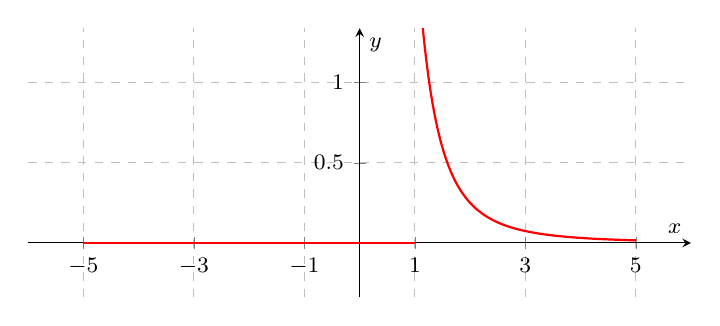
\begin{tikzpicture}
			\begin{axis}[
					font=\footnotesize,
					width=10cm,
					height=5cm,
					axis lines = center,
					xlabel = $x$,
					ylabel = $y$,
					xtick = {-5, -3, -1, 1, 3, 5},
					ytick = {0.5, 1},
					ymin = -0.2, ymax = 1.2,
					xmin = -5, xmax = 5,
					grid = both,
					grid style = dashed,
					legend pos = north west,
					enlargelimits
				]


				\addplot [
					domain=-5:1,
					samples=100,
					thick,
					color=red
				]
				{0};

				\addplot [
					name path=f,
					domain=1:5,
					samples=100,
					thick,
					color=red,
				]
				{2 * x^(-3)};
			\end{axis}
		\end{tikzpicture}
	\end{center}
	Nel grafico $\beta = 3$ ma, in generale, più $\beta$ è grande, più la funzione va velocemente
	a 0. Ecco che il parametro $\beta$ determina quanto la coda della distribuzione sia
	\emph{pesante} (valori bassi di $\beta$) o \emph{leggera} (valori alti di $\beta$).
	Verifichiamo ora il momento di ordine $n$ considerando $g(x) = |x|^n \geq 0$ e dunque
	\begin{align*}
		\E[g(x)] = & \int g(x) \cdot f(x) dx                              \\
		=          & \int_1^{+\infty} x^n \cdot (\beta - 1) x^{-\beta} dx \\
		=          & \int_{1}^{+\infty} (\beta-1) \cdot x^{-\beta+n} dx
	\end{align*}
	Ecco che qui abbiamo due possibili casi
	\[
		\E[g(x)] = \begin{cases}
			-\frac{\beta-1}{\beta-n-1} \cdot x^{-\beta+n+1} \Big|_1^{+\infty}
			                                          & -\beta+n+1 \neq 0 \\[2ex]
			(\beta-1) \cdot \log(x) \Big|_1^{+\infty} & -\beta+n+1=0
		\end{cases}
	\]
	Ecco che nel caso in cui $-\beta+n+1 < 0$ abbiamo che il valore atteso vale
	\[ \frac{\beta-1}{\beta-n-1} \]
	nel caso $-\beta+n+1 = 0$ abbiamo che $\log(+\infty) = +\infty$ e quindi il valore atteso è
	$+\infty$, nel caso di $-\beta+n+1 > 0$ abbiamo che l'esponente di $x$ nella della prima
	equazione e positivo e dunque, per $x \to +\infty$, il valore atteso è $+\infty$. Concludiamo
	che $X$ ammette momento di ordine $n$ se e solo se $-\beta+n+1 < 0$ ovvero se e solo se
	\[ n < \beta - 1 \]
	Deduciamo quindi che, quanto più grande è $\beta$ (e quindi quanto più sono leggere le code)
	tanti di più sono i momenti che possiamo ammettere.
\end{example}

\begin{proposition}
	Se $X$ ammette momento di ordine $n$, allora ammette momento di ordine $m$ per ogni $m \leq n$.
\end{proposition}

\begin{proposition}[Disuguaglianza di Markov]\label{prop: markov}
	Sia $X$ una variabile aleatoria a valori non negativi e sia $a>0$, allora
	\[ P(X > a) \leq \frac{\E[X]}{a} \]
	\begin{proof}
		Introduciamo la seguente variabile aleatoria $Z : \Omega \to \R$
		\[
			Z = \begin{cases}
				a & \text{su } \{ X > a \} \subseteq \Omega    \\
				0 & \text{su } \{ X \leq a \} \subseteq \Omega
			\end{cases}
		\]
		Vediamo che sull'insieme $\{ X > a \}$ abbiamo che $Z = a$ e, in particolare $Z \leq X$.
		Sull'altro insieme abbiamo che $Z = 0$ ma $X \geq 0$ e quindi $Z \leq X$ su $\Omega$.
		Vale quindi che
		\[ \E[X] \geq \E[Z] = a \cdot P(Z = a) + 0 \cdot P(Z = 0) = a \cdot P(X \geq a) \]
	\end{proof}
\end{proposition}

\begin{corollary}
	Se $X$ ammette momento di ordine $n$, allora
	\[ P(|X| > a) \leq \frac{\E[|X|^n]}{a^n} \]
	per ogni $a > 0$.
\end{corollary}

\begin{proposition}[Disuguaglianza di Schwartz]
	Siano $X$ e $Y$ due variabili aleatorie, allora
	\[ \E[|XY|] \leq \sqrt{\E[|X|^2]} \cdot \sqrt{\E[|Y|^2]} \]
	Possiamo dire che $X \cdot Y$ ammette valore atteso se $X$ e $Y$ ammettono momento secondo.
\end{proposition}

\begin{example}
	Consideriamo 2 lanci di un dado equilibrato e vogliamo calcolare i valori attesi di somma e
	prodotto. Chiamiamo $X$ l'esito del primo lancio e $Y$ l'esito del secondo lancio. Iniziamo
	con il calcolare il valore atteso della somma
	\[ \E[X + Y] = \E[X] + \E[Y] = \frac{7}{2} + \frac{7}{2} = 7 \]
	Calcoliamo ora il valore atteso del prodotto, assumendo che i lanci del dado siano prove
	ripetute indipendenti
	\[ \E[X \cdot Y] = \E[X] \cdot \E[Y] = \frac{7}{2} \cdot \frac{7}{2} = \frac{49}{4} = 12.25 \]
	Quando $X$ assume un numero finito di valori ammette momento di ogni ordine.
\end{example}

\begin{example}
	Sia $S$ una popolazione e sia $X : S \to \R$ una variabile che rappresenta un carattere
	discreto di un certo individuo della popolazione. L'estrazione di un individuo da $S$ è
	modellizzata dal modello uniforme, $\Omega = S$, $\F = \mathcal{P}(\Omega)$ e $P$ è uniforme.
	Abbiamo quindi che
	\[
		\E[X] = \sum_i x_i \cdot P(X = x_i) =
		\sum_i x_i \cdot \frac{\# \{\omega \in S | X(\omega) = x_i\}}{\# S}
	\]
	Questo equivale alla \textbf{frequenza relativa} di $X = x_i$ su tutta la popolazione e quindi
	$\E[X]$ è la media campionaria su tutta la popolazione e non su un singolo campione.
\end{example}

\subsection{Varianza}
D'ora in poi supporremo che le variabili aleatorie che trattiamo abbiano momento secondo.
Analogamente al caso della varianza in statistica descrittiva, la \textbf{varianza} di una
variabile aleatoria $X$ misura la \emph{dispersione} di $X$ attorno al valore atteso $\E[X]$. La
varianza di $X$ è la media pesata del quadrato degli scarti di $X$ da $\E[X]$.

\begin{definition}
	Data $X$ con momento secondo, si chiama \textbf{varianza} di $X$ la quantità
	\[ \Var(X) = \E[(X - \E[X])^2] \]
	Si chiama \textbf{scarto quadratico medio} o \textbf{deviazione standard} la quantità
	\[ \sigma(X) = \sqrt{\Var(X)} \]
\end{definition}

\begin{observation}
	La varianza di $X$ dipende solo dalla legge $P_X$.
\end{observation}

\begin{observation}
	Sviluppando il quadrato
	\[ (X - \E[X])^2 = X^2 + \E[X]^2 - 2 X \E[X] \]
	otteniamo
	\[ \Var(X) = \E[X^2] - \E[X]^2 \]
	Inoltre vale
	\[ \Var(aX + b) = a^2 \Var(X) \]
\end{observation}

\begin{example}
	Calcoliamo ora la varianza del lancio di un dado data la variabile $X$ che rappresenta l'esito
	di un lancio.
	\[ \Var(X) = \E[X^2] - \E[X]^2 = \frac{91}{6} - \left(\frac{7}{2}\right)^2 = \frac{35}{12} \]
\end{example}

\begin{proposition}[Disuguaglianza di Chebyshev]
	Sia $X$ con momento secondo e sia $d > 0$, allora
	\[ P(|X - \E[X]| \geq d) \leq \frac{\Var(X)}{d^2} \]
	possiamo vedere questo come una stima quantitativa della dispersione tramite la varianza.
	\begin{proof}
		Possiamo riscrivere il termine a sinistra dell'equazione precedente come
		\[ P(|X - \E[X]| \geq d) = P((X - \E[X])^2 \geq d^2) \]
		A questo punto, applicando la \hyperref[prop: markov]{disuguaglianza di Markov} otteniamo
		che
		\[ P((X - \E[X])^2 \geq d^2) \leq \frac{\E[(X - \E[X])^2]}{d^2} \]
		a questo punto usiamo la definizione di varianza per ottenere
		\[ \frac{\E[(X - \E[X])^2]}{d^2} = \frac{\Var(X)}{d^2} \]
	\end{proof}
\end{proposition}

In particolare, quest'ultimo risultato ci dice che se la varianza è nulla allora la variabile
aleatoria è costante a meno di un insieme trascurabile. Vale quindi
\[ \Var(X) = 0 \Longleftrightarrow X = k \]
dove $k$ è una costante e quindi vale anche
\[ \Var(X) = 0 \Longleftrightarrow P(X - \E[X] \neq 0) = 1 \]

\begin{example}
	Consideriamo una popolazione $S$ e $X : S \to \R$ (discreta) che rappresenta il carattere di un
	individuo della popolazione. In questo caso $\Var(X)$ è la varianza empirica ma su tutta la
	popolazione.
\end{example}
\section{Covarianza}
La covarianza entra in gioco quando si ha a che fare con variabili aleatorie doppie o, più in
generale, variabili aleatorie multiple.

\begin{definition}
	Date $X$ e $Y$ due variabili aleatorie con momento secondo, si chiama \textbf{covarianza} tra
	$X$ e $Y$ la quantità
	\begin{align*}
		\Cov(X, Y) = & \E[(X - \E[X]) \cdot (Y - \E[Y])] \\
		=            & \E[X \cdot Y] - \E[X] \cdot \E[Y]
	\end{align*}
\end{definition}

\begin{definition}
	Se $\Var(X) \neq 0$ e $\Var(Y) \neq 0$, si chiama \textbf{coefficiente di correlazione} la
	quantità
	\[
		\rho(X,Y) = \frac{\Cov(X, Y)}{\sigma(X) \cdot \sigma(Y)}
		= \frac{\Cov(X, Y)}{\sqrt{\Var(X) \cdot \Var(Y)}}
	\]
	Possiamo dire che quando $\rho(X,Y) = 0$ le due variabili $X$ e $Y$ sono \emph{scorrelate}.
\end{definition}

Di seguito elenchiamo alcune proprietà molto utili per la covarianza
\begin{itemize}
	\item $\Cov(aX + bY + c, Z) = a \cdot \Cov(X, Z) + b \cdot \Cov(Y, Z)$
	\item $\Cov(X,Y) = \Cov(Y,X)$ e $\Var(X) = \Cov(X, X)$
	\item $\Var(X+Y) = \Var(X) + \Var(Y) + 2 \cdot \Cov(X, Y)$
	\item $\rho(X,Y) = 0 \implies \Var(X + Y) = \Var(X) + \Var(Y)$
\end{itemize}

\begin{proposition}
	Date $X$ e $Y$ con momento secondo e tali che $\Var(X) \neq 0$ e $\Var(Y) \neq 0$, allora
	\begin{itemize}
		\item $|\rho(X,Y)| \leq 1$
		\item $\min_{(a,b) \in \R^2} (\E[(Y - a - bX)^2]) = \Var(Y) \cdot (1 - \rho(X,Y)^2)$
	\end{itemize}
\end{proposition}

Per capire meglio il secondo punto dobbiamo considerare $(a^*,b^*)$ che realizzano il minimo
nella seconda equazione, la retta $y = a^* + b^* X$ è la migliore approssimazione lineare tra
$X$ e $Y$. Stiamo cioè minimizzando la distanza tra $Y$ e $a+bX$. Il valore del minimo è
proporzionale a $1 - \rho(X,Y)^2$.

In altre parole, la relazione tra $X$ e $Y$ è tanto meglio approssimata dalla retta $y=a^*+b^*X$
quanto più $\rho$ è vicino a 1. In questo senso $rho$ è una misura della \textbf{dipendenza lineare}
tra $X$ e $Y$.

A questo punto dobbiamo stare attenti a non confonderci con l'indipendenza: se due variabili sono
indipendenti allora avranno una dipendenza lineare nulla $\rho=0$, ma in generale non è vero che
se $\rho=0$ allora le due variabili sono indipendenti (potrebbe esserci un'altra forma di
dipendenza).

\begin{proposition}
	Se $X$ e $Y$ sono indipendenti e hanno momento secondo, allora sono scorrelate. Il viceversa è
	in generale falso.
	\begin{proof}
		Se $X$ e $Y$ sono indipendenti vale
		\[ \Cov(X,Y) = \E[X \cdot Y] - \E[X] \cdot \E[Y] = 0 \]
		Per il viceversa serve un controesempio e nel nostro caso possiamo considerare
		$X \sim U([0,1])$ e $Y = X^2$. Si può verificare che $X$ e $Y$ sono scorrelate ma non sono
		indipendenti.
	\end{proof}
\end{proposition}
\section{Teoremi limite}
I \textbf{teoremi limite} entrano in gioco quando si vuole, in un certo senso, passare al lato
più empirico della statistica, ecco che vengono introdotti la \textbf{legge dei grandi numeri} e
il \textbf{teorema del limite centrale}.

Prendiamo per esempio il lancio di una moneta equilibrata. Se si effettuano 1000 lanci ci
aspettiamo di ottenere all'incirca 500 teste se la moneta è equilibrata. La legge dei grandi numeri
cerca di formalizzare questo risultato, mentre il teorema del limite centrale cerca di quantificare
le oscillazioni del numero di teste attorno a 500. Iniziamo però a dare qualche definizione.

\begin{definition}
	Data una famiglia di variabili aleatorie $X_1, X_2, \dots, X_n$ (possibilmente infinita), le
	variabili $X_i$ si dicono indipendenti e identicamente distribuite (i.i.d) se sono indipendenti
	e hanno la stessa distribuzione (cioè $P_{X_i}$ non dipende da $i$).

	Nel caso di famiglia infinita, diciamo che le $X_i$ sono indipendenti se $\forall n \in \N$ le
	variabili $X_1, X_2, \dots, X_n$ sono indipendenti.
\end{definition}

Dire che la variabile $X_i$ sono i.i.d equivale a dire che le $X_i$ hanno la stessa funzione di
ripartizione
\[ P(X_i \leq t) = F_{X_i} (t) = F(t) \]
per ogni $i$ e inoltre significa che sono indipendenti
\[ P(X_1 \leq t_1, \dots, X_n \leq t_n) = F_{X_1} (t_1) \cdot ... \cdot F_{X_n} (t_n) \]
per ogni $t_1, \dots, t_n \in \R$. Il tipico esempio di variabili aleatorie i.i.d è dato dalle
ripetizioni di un esperimento (non perforza con esisto successo o insuccesso).

Consideriamo $n$ (o anche infinite) ripetizioni di un esperimento nelle stesse condizioni. Sia
$X$ la variabile aleatoria che descrive un carattere dell'esperimento (ad esempio l'esito del
lancio di un dado). Per $i \in \N^+$, sia $X_i$ il valore del carattere dell'esito dell'$i$-esimo
esperimento. Allora le $X_i$ sono i.i.d.

Come caso particolare consideriamo l'estrazione di un campione da una popolazione reale.
Consideriamo quindi una popolazione e sia $X$ la variabile aleatoria che rappresenta un carattere
degli individui. Supponiamo ora di estrarre casualmente $n$ individui, in modo indipendente l'uno
dall'altro, e chiamiamo $X_i$ il carattere dell'$i$-esimo individuo estratto. Allora gli $X_i$
sono i.i.d con la stessa distribuzione di $X$.

Introduciamo ora la notazione per la media aritmetica di $n$ variabili aleatorie $X_1, \dots, X_n$
i.i.d
\[ \overline{X} = \overline{X_n} = \frac{X_1 + X_2 + \dots + X_n}{n} \]
Osserviamo che $\overline{X}$ è essa stessa una variabile aleatoria in quanto combinazione di
variabili aleatorie. Osserviamo anche che se $X_1, \dots, X_n$ rappresenta un campione,
$\overline{X}$ è la media campionaria del campione.

\begin{example}
	Consideriamo il caso di $n$ ripetizioni di un esperimento con esito successo o insuccesso.
	Chiamiamo $A$ il successo e sia $p = P(A)$ e sia $X_i$ la variabile aleatoria di Bernoulli
	associata all'$i$-esima ripetizione
	\[
		X_i = \begin{cases}
			1 & \text{se accade $A$ all'$i$-esima ripetizione} \\
			0 & \text{altrimenti}
		\end{cases}
	\]
	Allora le $X_i$ sono i.i.d indipendenti e con distribuzione $B(p)$, quindi $X=X_1+\dots+X_n$ è
	una variabile aleatoria $B(n,p)$ e rappresenta la \textbf{frequenza assoluta} del successo
	(di $A$) mentre
	\[ \overline{X} = \frac{X}{n} \]
	rappresenta la frequenza relativa del successo.
\end{example}

\subsection{Legge dei grandi numeri}
Uno degli obbiettivi fondamentali della legge dei grandi numeri è studiare il valore di
$\overline{X}$ per campioni grandi ($n$ grande). Questo significa calcolare in qualche modo il
limite, ma trattandosi di variabili aleatorie dobbiamo definire meglio cosa si intenda per limite.
Per la legge dei grandi numeri, ci serve la \textbf{convergenza in probabilità}.

\begin{definition}
	Una successione $Y_1, \dots, Y_n, \dots$ di variabili aleatorie definite sullo stesso spazio
	diciamo che \textbf{converge in probabilità} a una variabile aleatoria $Y$ se
	\[ P(|Y_n - Y| > \varepsilon) \to 0 \]
	per ogni $\varepsilon > 0$. In alternativa possiamo vedere la cosa in questo modo
	\[ \lim_{n \to +\infty} P(|Y_n - Y| > \varepsilon) = 0 \]
	Stiamo quindi dicendo che per $n$ grande $Y_n$ è vicina a $Y$ con probabilità alta.
\end{definition}

\begin{theorem}[Legge debole dei grandi numeri]
	Sia $X_1, \dots, X_n, \dots$ una successione di variabili aleatorie i.i.d dotate di momento
	secondo e sia $\mu = \E[X_i]$, allora $\overline{X}$ converge in probabilità a $\mu$, cioè
	\[ P(|\overline{X} - \mu| > \varepsilon) \to 0 \]
	per $n \to +\infty$ e per ogni $\varepsilon > 0$.
\end{theorem}

In altre parole il teorema dice che la media campionaria dei primi $n$ termini tende, per $n$
grande, al valore atteso. Valore atteso che è la media sulla popolazione nel caso di estrazione.


\include{inferenza/campioni_va}

\end{document}

